% LaTeX Template
% Version 1.3 (21/12/12)
%
% This template has been downloaded from:
% http://www.latextemplates.com
%
% Original authors:
% Steven Gunn 
% http://users.ecs.soton.ac.uk/srg/softwaretools/document/templates/
% and
% Sunil Patel
% http://www.sunilpatel.co.uk/thesis-template/
%
% License:
% CC BY-NC-SA 3.0 (http://creativecommons.org/licenses/by-nc-sa/3.0/)
%
% Note:
% Make sure to edit document variables in the Thesis.cls file
%
%%%%%%%%%%%%%%%%%%%%%%%%%%%%%%%%%%%%%%%%%

%----------------------------------------------------------------------------------------
%	PACKAGES AND OTHER DOCUMENT CONFIGURATIONS
%----------------------------------------------------------------------------------------

\documentclass[11pt, a4paper, oneside]{Thesis} % Paper size, default font size and one-sided paper

\usepackage[utf8]{inputenc}
\usepackage[section]{placeins}


\graphicspath{{./Pictures/}} % Specifies the directory where pictures are stored

\usepackage[square, numbers, comma, sort&compress]{natbib} % Use the natbib reference package - read up on this to edit the reference style; if you want text (e.g. Smith et al., 2012) for the in-text references (instead of numbers), remove 'numbers' 
\hypersetup{urlcolor=blue, colorlinks=true} % Colors hyperlinks in blue - change to black if annoying
\title{\ttitle} % Defines the thesis title - don't touch this

\begin{document}

\frontmatter % Use roman page numbering style (i, ii, iii, iv...) for the pre-content pages

\setstretch{1.3} % Line spacing of 1.3

% Define the page headers using the FancyHdr package and set up for one-sided printing
\fancyhead{} % Clears all page headers and footers
\rhead{\thepage} % Sets the right side header to show the page number
\lhead{} % Clears the left side page header

\pagestyle{fancy} % Finally, use the "fancy" page style to implement the FancyHdr headers

\newcommand{\HRule}{\rule{\linewidth}{0.5mm}} % New command to make the lines in the title page

% PDF meta-data
\hypersetup{pdftitle={\ttitle}}
\hypersetup{pdfsubject=\subjectname}
\hypersetup{pdfauthor=\authornames}
\hypersetup{pdfkeywords=\keywordnames}

%----------------------------------------------------------------------------------------
%	TITLE PAGE
%----------------------------------------------------------------------------------------




\begin{center}
\linespread{1.15}
\textbf{\large{UNIVERSIDAD TÉCNICA FEDERICO SANTA MARÍA\\}
\normalsize{DEPARTAMENTO DE ELECTRÓNICA\\VALPARAÍSO - CHILE\\}}

\vspace{0.5cm}
\begin{figure}[!ht]
\centering
  
\includegraphics[width=5.85cm]{./Figures/usmLogo.png}
\end{figure}
\vspace{0.5cm}

\linespread{1}\hangindent=0cm
\textbf{\Large ``DISEÑO Y CONSTRUCCIÓN DE PLATAFORMA PARA ESTUDIO DE ENJAMBRES DE ROBOTS''\\}
\vspace{3cm}

\hangindent=0cm\large \textbf{SEBASTIÁN IGNACIO SÁEZ SAN JUAN}\\
\vspace{0.5cm}
\hangindent=0cm\normalsize \textbf{MEMORIA DE TITULACIÓN PARA OPTAR AL TÍTULO DE INGENIERO CIVIL ELECTRÓNICO}\\
\vspace{3cm}

\vspace{0.5cm}
\begin{figure}[!ht]
\centering
  
\includegraphics[width=\textwidth]{./Figures/profesores.png}
\end{figure}
\vspace{0.5cm}

%\hangindent=0cm\normalsize \textbf{PROFESOR GUIA: \hspace{1cm} DRA. MARÍA JOSE ESCOBAR}\\
%\vspace{0.5cm}
%\hangindent=0cm\normalsize \textbf{PROFESOR CORREFERENTE: \hspace{1cm} DR. PABLO PRIETO}\\
%\vspace{0.5cm}
%\hangindent=0cm\normalsize \textbf{PROFESOR CORREFERENTE: \hspace{1cm} DR. JUAN CRISTOBAL ZAGAL}\\


\end{center}
%
%\begin{center}
%
%\textsc{\LARGE \univname}\\[1.5cm] % University name
%\textsc{\Large Memoria Titulación}\\[0.5cm] % Thesis type
%
%\HRule \\[0.4cm] % Horizontal line
%{\huge \bfseries \ttitle}\\[0.4cm] % Thesis title
%\HRule \\[1.5cm] % Horizontal line
% 
%\begin{minipage}{0.4\textwidth}
%\begin{flushleft} \large
%\emph{Autor:}\\
%\end{flushleft}
%\end{minipage}
%\begin{minipage}{0.4\textwidth}
%\begin{flushright} \large
%\emph{Supervisores:} \\
%\end{flushright}
%\end{minipage}\\[3cm]
% 
%\large \textit{Memoria para optar al grado de \degreename}\\[0.3cm] % University requirement text
%\textit{en el}\\[0.4cm]
%\deptname\\[2cm] % Research group name and department name
% 
%{\large \today}\\[4cm] % Date
%%\includegraphics{Logo} % University/department logo - uncomment to place it
% 
%\vfill
%\end{center}



%----------------------------------------------------------------------------------------
%	DECLARATION PAGE
%	Your institution may give you a different text to place here
%----------------------------------------------------------------------------------------



%----------------------------------------------------------------------------------------
%	QUOTATION PAGE
%----------------------------------------------------------------------------------------



%----------------------------------------------------------------------------------------
%	ABSTRACT PAGE
%----------------------------------------------------------------------------------------

\addtotoc{Resumen} % Add the "Abstract" page entry to the Contents

\resumen{\addtocontents{toc}{\vspace{1em}} % Add a gap in the Contents, for aesthetics
Desarrollo de una plataforma, de bajo costo, que permita estudiar el comportamiento de grupos de robots. Para que la plataforma funcione es necesario el diseño y construcción de los robots , implementar sistema de tracking 2D, armar la red de comunicación (XBee) y construir el software de control.
}

\clearpage % Start a new page


%----------------------------------------------------------------------------------------
%	ABSTRACT PAGE
%----------------------------------------------------------------------------------------

\addtotoc{Abstract} % Add the "Abstract" page entry to the Contents

\abstract{\addtocontents{toc}{\vspace{1em}} % Add a gap in the Contents, for aesthetics
Create a low cost platform, which allows to study the behavior of a group of robots. For this platform to work, it is necessary the design and building of the robots, implement a 2D tracking system, build a communication network (xbee) and create the control software.
}

\clearpage % Start a new page

%----------------------------------------------------------------------------------------
%	ACKNOWLEDGEMENTS
%----------------------------------------------------------------------------------------

\setstretch{1.3} % Reset the line-spacing to 1.3 for body text (if it has changed)

\acknowledgements{\addtocontents{toc}{\vspace{1em}} % Add a gap in the Contents, for aesthetics 

Este trabajo no habría podido realizarse sin el apoyo incondicional de mi profesora tutora, Dra. María José Escobar que ha tenido una gran paciencia conmigo y siempre me ha ayudado en lo posible. También fue fundamental el apoyo del Dr. Juan Cristóbal Zagal que gentilmente me permitió trabajar en su innovador laboratorio de Síntesis de máquinas inteligentes. No menos importante fue el apoyo del Dr. Pablo Prieto que ha sido un guía para mí en el diseño del robot. Además de ellos conté con la ayuda de muchas personas que han dedicado parte de su tiempo a escuchar mis ideas y aconsejarme. Es por esto que quiero agradecer a Jaime Martínez por ayudarme a diseñar el PCB de MODI, Carlos Galáz por sus inacabables minutos telefónicos para discutir casi todos los aspectos de MODI, Fabián Rubilar por sus ideas de como mover los robots, Linus Casassa por su paciencia para explicarme cualquier cosa sobre electrónica, la gente del taller de electrónica por enseñarme a soldar y sacarme de apuros técnicos, Ricardo Pérez por las interminables discusiones sobre el robot, mis compañeros del laboratorio de Sintesís de máquinas inteligentes y a mi amada Pía que siempre ha estado ahí conmigo siendo un gran apoyo en mi vida.
}
\clearpage % Start a new page

%----------------------------------------------------------------------------------------
%	LIST OF CONTENTS/FIGURES/TABLES PAGES
%----------------------------------------------------------------------------------------

\pagestyle{fancy} % The page style headers have been "empty" all this time, now use the "fancy" headers as defined before to bring them back

\lhead{\emph{Contents}} % Set the left side page header to "Contents"
\tableofcontents % Write out the Table of Contents

\lhead{\emph{Índice de Figuras y Tablas}} % Set the left side page header to "List of Figures"
\listoffigures % Write out the List of Figures


%----------------------------------------------------------------------------------------
%	DEDICATION
%----------------------------------------------------------------------------------------

\setstretch{1.3} % Return the line spacing back to 1.3

\pagestyle{empty} % Page style needs to be empty for this page

\dedicatory{Pía, mi fiel compañera de aventuras\ldots} % Dedication text

\addtocontents{toc}{\vspace{2em}} % Add a gap in the Contents, for aesthetics
\addcontentsline{toc}{chapter}{Prefacio}

%----------------------------------------------------------------------------------------
%	THESIS CONTENT - CHAPTERS
%----------------------------------------------------------------------------------------

\mainmatter % Begin numeric (1,2,3...) page numbering

\pagestyle{fancy} % Return the page headers back to the "fancy" style

% Include the chapters of the thesis as separate files from the Chapters folder
% Uncomment the lines as you write the chapters


% Prefacio

\chapter*{Prefacio} % Main chapter title

\label{Prefacio} % For referencing the chapter elsewhere, use \ref{Chapter1} 

\lhead{Prefacio} % This is for the header on each page - perhaps a shortened title

%----------------------------------------------------------------------------------------
A comienzos de la década de 1990, siendo todavía yo un niño, me escondía en la logia de la casa de mis padres, que estaba ubicada en la comuna de Ñuñoa, a desarmar cuanto artefacto cayera en mis manos. Según recuerdo, sumado a lo que mi madre me ha contado, una vez desarmé el único teléfono que había en la casa. Era uno de esos que ya no se ven, que hacen uso de un dial para marcar el número. Tal era mi curiosidad sobre esta máquina, que la desarmé completamente, solo para tratar de entender como se producía ese sonido sin igual que llamaba la atención de toda persona que estuviera en la casa. Por supuesto mi madre me retó porque no pude volver a armarlo, pero en secreto siempre supe que ella y mi padre se divertían con mis pequeñas aventuras. En esta misma casa, mi padre intentó montar una empresa de consultores con unos amigos, lo que significaba que al lado de mi pequeño taller clandestino tenía a mi disposición tres o cuatro computadores con sus flamantes pantallas Hércules frente a la cuales pasé tardes completas jugando los primeros vídeo juegos, y sin darme cuenta fue así como di mis primeros pasos en la computación. Algo más grande, cuando tenía 13 años, por el trabajo de mi padre nos fuimos a vivir a Concepción. Una ciudad bien particular, ya que el invierno da mucho tiempo para estar en el hogar. Ahí volví a encontrarme con la computación. Recuerdo que mientras mis compañeros estaban en clases, yo me escabullía para ir directo a las salas de computación, donde el encargado me permitía ayudarle a instalar Windows 95 en los computadores. Disquete tras disquete instalábamos el programa en cada computador hasta lograr que el famoso logo de la ventana saliera en la pantalla. Desde esa  época es que familiares y amigos me han pedido ayuda con sus máquinas. En la enseñanza media volvimos como familia a Santiago, volví a mi colegio de infancia, el Liceo San Agustín. Por ese tiempo junto a dos compañeros nos inscribimos en el concurso escolar de robótica de la Universidad Diego Portales. Aquí alumnos de la mencionada universidad nos enseñaron como se podía construir y programar un robot. No fue fácil y luego de un par de meses entre tantos manuales y simbología alienígena (diagramas eléctricos) tomamos la decisión de retirarnos. En el año 2005 ingresé a la Universidad Técnica Federico Santa María (USM). Llegué el 2006 a Valparaíso y lo primero que vi en el patio central fue un pequeño cartel que decía: "Taller del Centro de Robótica", junto a otro amigo que hice apenas ingresé a la USM, entusiasmados con esta idea de hacer nuestros propios robots, no lo dudamos y nos inscribimos para ser parte de ese taller. Una vez dentro del Centro de Robótica, conocí mucha gente con intereses similares a los míos, con gran conocimiento y más que nada, una gran solidaridad para compartir éste. Tardes completas dedicadas a aprender las oscuras artes de la electrónica, luchando con la frustración de armar un circuito y que éste no funcionara a la primera, fui paso a paso avanzando hasta poder construir mis primeros robots. Argo fue el primer proyecto de robótica en que me incluí, donde se trataba de construir un robot cuadrúpedo capaz de moverse en todas las direcciones en un plano utilizando la menor cantidad posible de grados de libertad. Luego vino LALO, proyecto que se destacó por ser de los primeros robots en hacer uso de un Smartphone como cámara y controlador de motores. En la actualidad me interesa más poder transmitir los conocimientos que tengo para introducir a la gente en las nuevas tecnologías existentes que están al alcance de todos.

Hacer Robots en Valparaíso no es una tarea sencilla, la falta de lugares especializados para comprar dificulta contar con los componentes necesarios para construir una máquina. Aunque no es imposible, a continuación explico como se hizo.



%----------------------------------------------------------------------------------------
% Chapter 1

\chapter{Introducción} % Introduccion al trabajo

\label{Chapter1} % For referencing the chapter elsewhere, use \ref{Chapter1} 

\lhead{Capítulo 1. \emph{Introducción}} % This is for the header on each page - perhaps a shortened title

%----------------------------------------------------------------------------------------
%--------------------------------------------------------
%Sección 1
%--------------------------------------------------------


\begin{figure}[htbp]
	\centering
		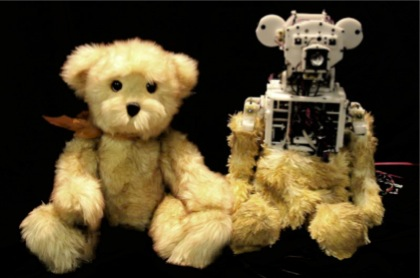
\includegraphics[width=0.8\textwidth]{./Figures/robot.jpg}
		%\rule{35em}{0.5pt}
%	\caption[Robot Huggable]{Robot creado por MIT Media Lab para cuidados personales. Imagen tomada de \cite{Stiehl:2006:HTR:1179133.1179149}}
	\label{fig:Huggable}
\end{figure}

La robótica es una rama de la tecnología que cada vez toma más importancia. Gracias a sus avances podemos construir complejas máquinas que nos asisten en tareas imposibles para nosotros los seres humanos y también nos permite estudiar la naturaleza al poder reproducir ciertos aspectos de ella con estas maquinas. Un aspecto que ultimamente a llamado la atención de los investigadores es, como los sistemas complejos existente en la naturaleza son capacez de llevar a cabo tareas que cada uno de sus individuos de forma aislada no pueden realizar. Actualmente existen investigadores que por medio de robots simples han logrado reproducir comportamientos colectivos como los observados en hormigas y otros animales. En Chile aún hay muy pocos grupos de investigación que centren sus trabajos en este tema, y es necesario contar con robots de bajo costo que faciliten la construcción de grupos de robots.

El trabajo se centró en la investigación de las tecnologías existentes para diseñar un robot que sea económico, simple y que de manera inalámbrica permita su control. El robot debe tener estas características ya que se necesita construir un enjambre para poder realizar estudios en el comportamiento y control de éstos.

Al comienzo de este proyecto se trabajó en Santiago de Chile, en conjunto con la Universidad de Chile (UChile) bajo la tutela del Doctor Juan Cristóbal Zagal en el Laboratorio de Síntesis de Máquinas Inteligentes. Por parte de la Universidad Técnica Federico Santa María (USM), se trabajó con la Doctora María José Escobar, del Departamento de Electrónica y luego se incorporó el Doctor Pablo Prieto del Departamento de Diseño de Productos. El financiamiento para realizar este prototipo ha sido por parte de las dos Instituciones, Universidad Técnica Federico Santa María y Universidad de Chile.

Durante el proceso de desarrollo se tuvieron que hacer diversas compras de materiales, pero los lugares más recurrentes al momento de hacerlas fueron Olimex y Casa Royal. La primera es una empresa dedicada a traer productos para hacer prototipos y construir máquinas, la segunda cuenta con varios insumos básicos para trabajar en desarrollo de circuitos electrónicos. Ambas empresas se encuentran en Santiago, por lo que trabajar en esta ciudad es de gran ayuda para reducir los tiempos en desarrollo.
Luego de armar un primer robot funcional, con materiales disponibles en Santiago de Chile, se hizo una búsqueda en internet de componentes en tiendas especializadas.

Este documento resume el desarrollo del proyecto MODI (Modular Intelligence), que es un robot simple de construir que tiene como fin ser repetible para facilitar la construcción de Enjambres de robots. En el capítulo 2 se explica lo que es un robot, algo de historia y algunos tipos de robots. El capítulo 3 comienza con un explicación sobre los enjambres de animales, luego se describen los robots usados actualmente en la literatura para estudiar enjambres y al final se describen las necesidades de mercado y las ventajas del proyecto MODI. El capítulo 4 está centrado en el diseño y herramientas de fabricación utilizadas durante el proceso de desarrollo. El capítulo 5 es el principal, describe criterios de diseño y el detalle de todos los componentes utilizados en el robot diseñado. Además se explica el software utilizado y el sistema que permite hacer un seguimiento de cada robot de forma individual. En el capítulo 6 se explican algunos posibles usos de los enjambres de robots. Al final, el capítulo 7 tiene sugerencias para mejoras futuras y las conclusiones. 

Para el comienzo de cada capítulo se escogío una imagen representativa que, por la diagramación escogida van sin leyenda. Estas imagenes son: Capítulo 1. Huggable, robot desarrollado por MIT para el cuidado y educación de niños; Capítulo 2. Digesting Duck, imagen perteneciente al dominio publico; Capítulo 3. Bandanda de Auklet, imagen perteneciente al dominio publico; Capítulo 4. Función matemática madera, diseñada por FabLab Barcelona; Capítulo 5. Robot MODI, robot diseñado en este trabajo.


%---------------------------------------------------------------------------------------- 


% Chapter 1

\chapter{Robot} % Main chapter title

\label{Chapter2} % For referencing the chapter elsewhere, use \ref{Chapter1} 

\lhead{Capítulo 2. \emph{Robot}} % This is for the header on each page - perhaps a shortened title

%----------------------------------------------------------------------------------------

%--------------------------------------------------------
%Sección 1
%--------------------------------------------------------

\begin{figure}[htbp]
	\centering
		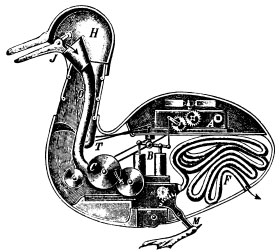
\includegraphics[width=0.6\textwidth]{./Figures/Duck_of_Vaucanson.jpg}
	%	\rule{35em}{0.5pt}
	%\caption[Robot Digesting Duck]{Digesting Duck, creado por Jacques de Vaucanson en 1739. Imagen tomada de Wikipedia.}
	\label{fig:Duck}
\end{figure}

Los robots ya son parte de la cultura pop, todos tienen al menos una idea de qué es un robot por la ciencia ficción o alguna noticia sobre los últimos avances. Incluso ya hay hogares en Chile que tienen una pequeña Robotina que recorre metódicamente todos los espacios de la casa para mantenerla sin polvo. A continuación un poco de historia y conceptos básicos de un robot.

\section{¿Qué es un robot?}

Un robot puede ser un software solamente o tener además una extensión física que le permita desempeñar tareas realizadas por el ser humano o que necesitan algo de inteligencia. El término robot se le atribuye al dramaturgo checo Karel Čapek, que en su obra R.U.R en 1921 (Rossum’s Universal Robots) utilizó la palabra \textit{robotnik} para referirse a ayudantes artificiales. Luego fue el escritor Isaac Asimov (1920-1992) quien,  gracias a su obra, difundió la palabra robótica haciendo referencia a la ciencia encargada de estudiar a los robots. Desarrolló las tres leyes de la robótica, que son una especie de normativa que regula el comportamiento de los robots en sus libros de Ciencia Ficción. Aparecidas por primera vez en el relato Runaround (1942), establecen lo siguiente:

\begin{enumerate}
\item Un robot no puede hacer daño a un ser humano o, por inacción, permitir que un ser humano sufra daño.
\item Un robot debe obedecer las órdenes dadas por los seres humanos, excepto si estas órdenes entrasen en conflicto con la 1ª Ley.
\item Un robot debe proteger su propia existencia en la medida en que esta protección no entre en conflicto con la 1ª o la 2ª Ley.
\end{enumerate}
La robótica como ciencia contempla el estudio de al menos seis áreas: La mecánica, la electrónica, la informática, el control automático, la física y la matemática.

Existen diferentes tipos y clases de robots, entre ellos con forma humana, de animales, de plantas. Todos se diferencian por sus capacidades y se clasifican en 4 formas:\begin{itemize}
\item Androides: robots con forma humana. Imitan el comportamiento de las personas, su utilidad en la actualidad es de solo experimentación. La principal limitante de este modelo es la implementación del equilibrio en el desplazamiento, pues es bípedo.
\item Móviles: se desplazan mediante una plataforma rodante (ruedas); estos robots aseguran el transporte de piezas de un punto a otro.
\item Zoomórficos: es un sistema de locomoción imitando a los animales. La aplicación de estos robots sirve, sobre todo, para el estudio de volcanes y exploración espacial.
\item Poliarticulados: mueven sus extremidades con pocos grados de libertad. Su principal utilidad es industrial, para desplazar elementos que requieren cuidados.
\end{itemize}

En ésta última se puede clasificar según su morfología en: Robots angulares o antropomórficos, robots cilíndricos, robots esféricos o polares, robots tipo SCARA, robots paralelos, robots cartesianos, entre otros. En este trabajo nos vamos a centrar solo en los robots Móviles con 2 ruedas.

En la historia hay varios intentos por construir estos ayudantes artificiales. A principios del siglo XVIII, Jacques de Vaucanson creó un autómata capaz de tocar la flauta, así como un pato mecánico que continuamente seguía su ciclo biológico.

En la actualidad las empresas KUKA, Honda y Sony, entre otras, construyen robots especialmente diseñados para la industria. Los robots que se utilizan en la industria, y los pocos que han llegado al hogar, son controlados por un algoritmo. Este es parte de un software que escribe una persona, donde se detalla la tarea que el robot debe realizar; tiene un modelo de los motores, partes y piezas para que así la máquina tenga información de como es, y pueda ejecutar la tarea para la cual se le programó. Si se interfiere con el entorno del robot, por ejemplo moviendo 1 [cm], fuera del rango de los sensores, el perno que debe apretar algún robot industrial que ensambla autos, este no podrá \textit{encontrarlo}. No todos los robots comerciales que existen hoy en día son capaces de adaptarse a cambios en el entorno (hay algunos que poseen sistemas de visión que permiten hacer estas correcciones), y menos ser capaces de generar una imagen de sí mismos que les permita entender qué sucede y recuperarse de fallas. Además de estos robots industriales hay algunos que son para uso militar que permiten desactivar bombas y rescatar personas. También existen robots que son capaces de asistir a una persona con discapacidades o incluso un robot acuático con una cámara que puede permitir a una persona recorrer el fondo del océano. 

\begin{figure}[htbp]
	\centering
		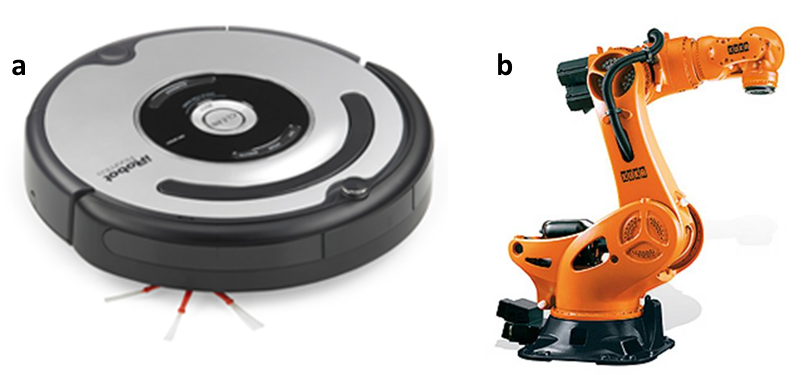
\includegraphics[width=\textwidth]{./Figures/RobotsInd.png}
		\rule{35em}{0.5pt}
	\caption[Robots Roomba y KUKA]{\textbf{a. }Robot Roomba, primer Robot doméstico vendido en Chile. Imagen tomada de \cite{Forlizzi:2006:SRD:1121241.1121286} \textbf{b.} Robot industrial KUKA KR 1000 TITAM. Imagen tomada de kuka-robotics.com}
	\label{fig:Roomba y KUKA}
\end{figure}

Para que un robot pueda hacer cosas es necesario programar el software de control. Se debe tener un modelo detallado de los motores y sensores que se poseen y es tarea del programador hacer la abstracción necesaria para poder darle sentido al movimiento del conjunto de motores. Cada motor aporta con un grado de libertad, o por su sigla en ingles DOF (degree of freedom), ver Figura \ref{fig:grados de libertad}. Los Grados de libertad hacen referencia al número de movimientos independientes que se pueden realizar. En otras palabras, un grado de libertad es la capacidad de moverse a lo largo de un eje (movimiento lineal) o de rotar en torno a un eje (movimiento rotacional). Por ejemplo, un auto posee 3 grados de libertad, dos de posición y uno de orientación. 

Si hablamos de un robot de 4 extremidades, con 3 grados de libertad en cada una, el programador debe ser capaz de indicar la secuencia de activación de cada motor. Primero debe hacer que el robot mueva una extremidad y luego con la suma de las 4 lograr desplazarse. Estamos hablando de 12 motores que pueden moverse de forma independiente, lo cual genera infinitas soluciones y no todas posibles debido a las restricciones físicas de la construcción misma del robot.

\begin{figure}[htbp]
	\centering
		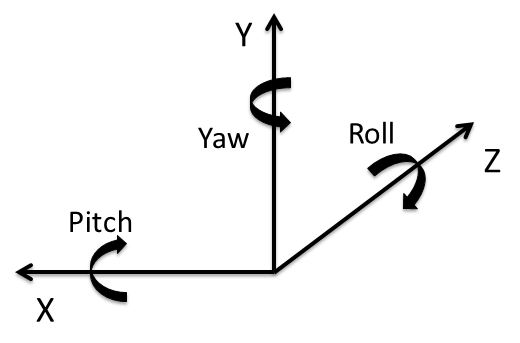
\includegraphics[width=\textwidth]{./Figures/6DOF.png}
		\rule{35em}{0.5pt}
	\caption[Grados de libertad]{Cada motor en un robot aporta un grado de liberdad. Acá hay seis grados de libertad, tres son de desplazamiento y tres son de orientación.}
	\label{fig:grados de libertad}
\end{figure}

Para programar el movimiento un robot cuadrúpedo es útil observar a la naturaleza, buscar animales que tengan una forma similar y tratar de replicar su movimiento. En ese sentido la naturaleza siempre ha sido una gran fuente de inspiración para las creaciones del ser humano. Actualmente el interés se ha volcado a investigar los enjambres de animales, que aunque están compuestos por muchos individuos de comportamiento simple son capaces de organizarse de alguna manera para cumplir con tareas más complejas. Entender y aplicar este tipo de comportamientos a grupos de robots puede ser de gran ayuda para cumplir con tareas distribuidas donde no sea suficiente el trabajo de un solo robot, si no más se requiera el trabajo de varios.



% Chapter Template

\chapter{Swarm} % Main chapter title

\label{Chapter3} % Change X to a consecutive number; for referencing this chapter elsewhere, use \ref{ChapterX}

\lhead{Capítulo 3. \emph{Swarms}} % Change X to a consecutive number; this is for the header on each page - perhaps a shortened title

\begin{figure}[htbp]
	\centering
		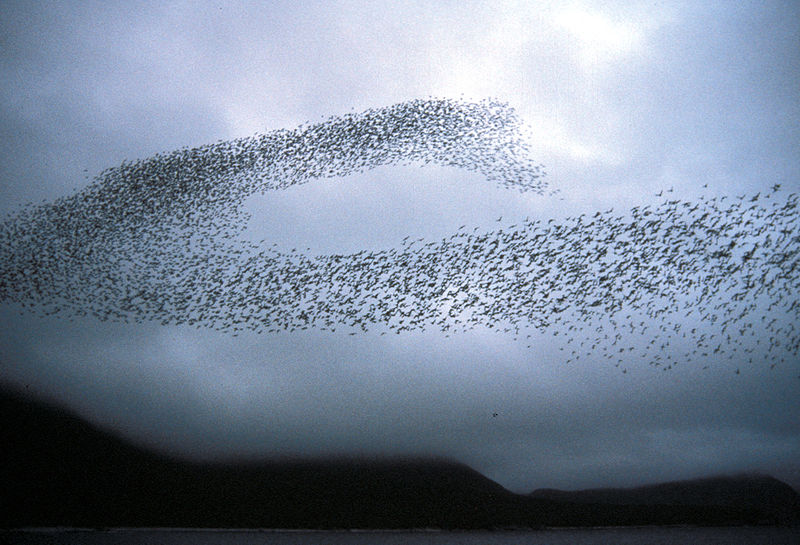
\includegraphics[width=0.8\textwidth]{./Figures/swarm.jpg}
	%	\rule{35em}{0.5pt}
	%\caption[Bandada de auklets]{Bandada de auklets teniendo comportamiento de enjambre. Imagen tomada de Wikipedia.}
	\label{fig:Bandada}
\end{figure}

El comportamiento colectivo de sistemas descentralizados, auto-organizados es llamado Inteligencia de Enjambre. Estos sistemas están formados típicamente por una población de individuos simples que interactúan entre ellos localmente y con su medio ambiente. Estos individuos siguen reglas muy simples, y pese a no tener una estructura de control centralizado que dicte cómo deben comportarse individualmente,  las interacciones entre los individuos conducen a la aparición de cierta inteligencia en el comportamiento global.

%----------------------------------------------------------------------------------------
%	SECTION 1
%----------------------------------------------------------------------------------------

\section{Comportamiento colectivo en la naturaleza}



En la naturaleza existen diversos casos de comportamiento colectivo. Los enjambres más típicos son las hormigas y abejas, pero los hay en peces, aves e incluso los mamíferos. Son sistemas donde nadie está a cargo y aún así ejecutan una tarea grupal. Las hormigas son un gran ejemplo. Al momento de construir su madriguera, no tienen un arquitecto o ingeniero estructural que esté dando órdenes, simplemente cada una sabe qué tiene que hacer. No hay un director orquestando la construcción desde lo alto, en vez de esto lo que ocurre es un comportamiento emergente. También conocido como inteligencia de enjambre\cite{bonabeau1999swarm}.

Otro tipo de comportamiento colectivo son las migraciones, desplazamientos periódicos que efectúan aves, peces, langostas y mamíferos de un hábitat a otro. Cada individuo activo en la migración sigue al grupo, los más pequeños como el plancton o anfibios aprovechan las corrientes de aire o agua, y las aves, más grandes, aprovechan los vientos y corrientes ascendentes. Hay diversas finalidades detrás de la migración, algunas especies lo hacen para escaparse de los crudos inviernos o secos veranos; mientras que otras, como las tortugas marinas, por una necesidad reproductiva emprenden un largo viaje de más de 10.000 millas, a lo largo de todo el Atlántico Norte.

Lograr que un enjambre de robots tenga un comportamiento emergente como el de las colonias de abejas es lo que están buscando investigadores de esta área. Uno de los más destacados investigadores del área James McLurkin, experto en robótica del Massachusetts Institute of Technology (MIT), dice que para lograrlo es necesario un software que ejecute tareas individuales y que de alguna forma se cumpla con una tarea grupal \cite{mclurkin2007distributed}. He aquí una importante razón para desarrollar estudios sobre enjambres de robots, ya que aún no está claro cómo se coordina la naturaleza para llevar a cabo tales tareas. Un ejemplo es el algoritmo Optimización de colonia de hormigas, que es una clase de algoritmos inspirado en las acciones de una colonia de hormigas y como hacen uso de la feromona. Su principal uso es en problemas donde se necesite encontrar caminos hacia una meta, simulando las feromonas para dirigir a cada uno de los individuos en la búsqueda. Utilizando este tipo de estrategia es posible que en un futuro no muy lejano se pueda utilizar para controlar nanobots dentro del cuerpo con el fin de eliminar los tumores del cáncer.

%-----------------------------------
%	SECTION 2
%-----------------------------------
\section{Robots para construir un enjambre}

Diferentes laboratorios del mundo han desarrollado robots que funcionan como enjambre, con diseños que satisface sus propios requerimientos. Dependiendo de ellos varían en costo, tamaño y funcionalidad.

Algunos robots que pueden ser utilizados para hacer un Robot Swarm junto con las información técnica disponible, son listados en la sub secciones siguientes.

%-----------------------------------
%	SUBSECTION 1
%-----------------------------------
\subsection{Kilobot}
El proyecto Kilobot, ver Figura \ref{fig:robots estudiados} a, es un sistema de bajo costo escalable para demostrar comportamientos colectivos. Actualmente el grupo Self-organizing Systems Research Group \footnote{http://www.eecs.harvard.edu/ssr/index.html} , de la Universidad de Harvard, está investigando algoritmos para enjambres de robots, por esto diseñó Kilobot, que es un robot de bajo costo, accesible,  que permite hacer pruebas en cientos o miles de robots. Con estos robots investigan temas como: encontrar "alimento" de forma grupal, seguir al líder y dispersarse unos de otro. Su principal característica es que son muy pequeños y simples de usar. Las desventajas de Kilobots son: su sistema de locomoción que obliga a tener una superficie extremadamente lisa para usarlos y que no poseen sistema de radio que permita en control de forma inalámbrica, solo comunicación local.

%-----------------------------------
%	SUBSECTION 2
%-----------------------------------
\subsection{Organismo Multibot}
S. Kornienko et al. \cite{5359578}, exploran el trabajo colaborativo en robots para un mejor rendimiento y mayor fiabilidad a nivel macroscópico. En este artículo demuestran sus últimos trabajos en sistemas colectivos y lo más sorprendente es que logran la agregación y desagregación autónoma para así obtener un organismo multibot. Este robot tiene la ventaja de tener un mecanismo que le permite unirse mecánicamente, pero también puede compartir energía, sensores y lógica con otros robots iguales para formar un organismo que es capaz de modificar su estructura y adaptarse al entorno auto-organizándose. En la Figura \ref{fig:robots estudiados} b, se puede ver una estructura formada por los robots. De los robots estudiados este es el único que posee esta capacidad de unirse de manera autónoma ya que su hardware fue concebido para tales fines, pero no representa una ventaja porque se acotó la búsqueda a robots con desplazamiento diferencial. Estos robots no cuentan con documentación detallada ni distribuidores que los vendan, al parecer están descontinuados.

%-----------------------------------
%	SUBSECTION 3
%-----------------------------------
\subsection{e-puck}
Uno de los robots más utilizados por los científicos en el mundo para estudios y publicaciones es el e-puck \cite{mondada2009puck}. Este robot es compacto, tiene forma de cilindro con un diámetro de 7 [cm] y para moverse hace uso de sus dos ruedas, dejándolo en la categoría de robot con desplazamiento diferencial. Originalmente fue diseñado para educar en el área de la micro ingeniería por Michael Bonani y Francesco Mondala en el laboratorio ASL del Profesor Roland Siegwart en Escuela Politécnica Federal de Lausana (EPFL) en Suiza. El e-puck es open hardware, su software es de código abierto,  lo construyen y venden varias empresas. Para comunicarse con un computador incorporan un módulo Bluetooth conectado a uno de sus dos puertos serie. Existen varios tipos de accesorios, entre los que destacan un Zigbee para comunicaciones, un módulo con varias cámaras y LEDs RGB como sistema de comunicación visual. Su principal desventaja es el alto precio y por lo mismo su uso está algo descontinuado. Además son complejos de programar y se necesita una licencia especial para su software.

%-----------------------------------
%	SUBSECTION 4
%-----------------------------------
\subsection{3pi Robot}

El 3pi fue diseñado especialmente como un robot seguidor de líneas y capaz de solucionar laberintos. Existen varios vídeos que muestran la asombrosa velocidad de estos robots para solucionar un laberinto \footnote{http://www.pololu.com/catalog/product/975}. Se programa en C, pero como posee un microcontrolador ATmega es posible hacer uso del bootloader Arduino y programarlo con ese IDE. Usa 4 baterías AAA y trae 4 LEDs.  Yi-Jen Mon1 utilizó estos robots para desarrollar Supervisory Adaptive Network-Based Fuzzy Inference System (SANFIS) de forma empírica en un robot móvil, no simulado en un computador. Sus desventajas son: No cuenta con un sistema de carga autónoma, hardware extra que no va ser necesario para nuestros experimentos, necesita un cable especial para programarlo y no tiene comunicación inalámbrica.


\begin{figure}[htbp]
	\centering
		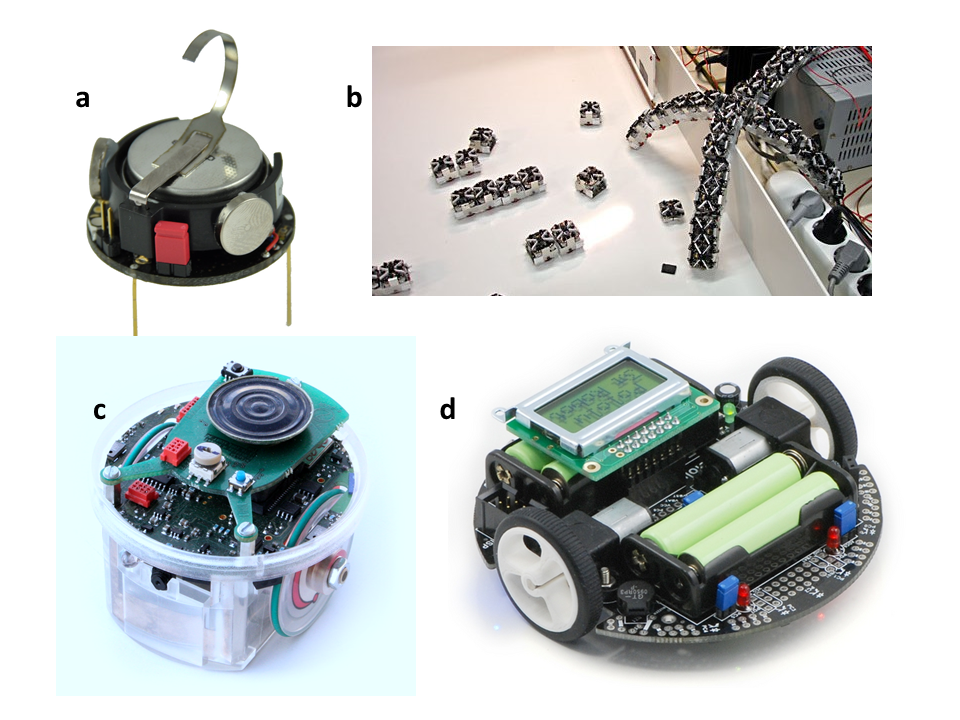
\includegraphics[width=\textwidth]{./Figures/robots1.png}
		\rule{35em}{0.5pt} 
	\caption[Robots estudiados como alternativa para armar un enjambre de robots.]{\textbf{a.} Kilobot, el más simple de todos y pequeño. Imagen tomada de \cite{6224638}. \textbf{b.} Organismo Multibot, permite armar estructuras con los robots. Imagen tomada de \cite{5359578}. \textbf{c.} e-puck, robot altamente difundido en investigaciones, caro y complejo. Imagen tomada de \cite{mondada2009puck}. \textbf{d.} 3pi Robot, simple y económico pero no tiene comunicación inalámbrica. Imagen tomada de \cite{thurskyusing}}
	\label{fig:robots estudiados}
\end{figure}

En la Figura \ref{fig:Tabla robots} hay una tabla comparativa que resume las principales características de los robot: Kilobot\footnote{http://www.k-team.com/mobile-robotics-products/kilobot/specifications}, e-puck\footnote{http://www.gctronic.com/doc/index.php/E-Puck} y 3pi\footnote{http://www.pololu.com/catalog/product/975/specs}. Lamentablemente para el multibot no es mucha la información disponible.


\begin{figure}[htbp]
	\centering
		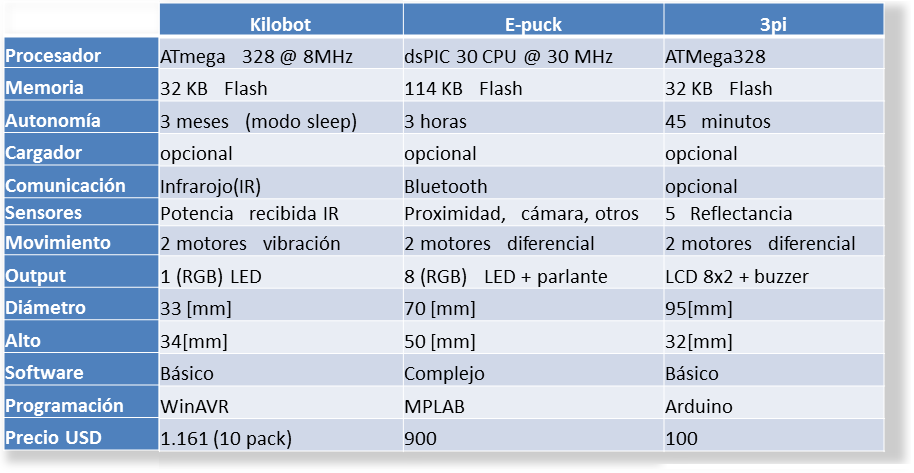
\includegraphics[width=1\textwidth]{./Figures/tabla_robots.png}
		\rule{35em}{0.5pt}
	\caption[Tabla comparativa robots]{En esta tabla se comparan las características principales de los robots: kilobot, e-puck y 3pi. No se incluyó el robot utilizado para el organismo multibot ya que no se comercializa.}
	\label{fig:Tabla robots}
\end{figure}

En esta tabla se comparan tres robots que pueden usarse para hacer estudios de enjambres de robots. De acá se resume que kilobot es un robot simple que no tiene comunicación inalámbrica, E-puck es un robot sumamente completo con un alto costo y está sobredimencionado para los estudios que se quieren hacer. El que más se acerca a nuestros requerimientos es el 3Pi de Pololu, pero cuenta con hardware extra que aumenta su consumo energético y no incorpora ningún sistema de comunicación inalámbrica.

\FloatBarrier
Además existen otros robots que podrían utilizarse en este trabajo, pero que al momento del desarrollo no existian. En el repositorio de objetos 3D de MakelBot Thingiverse existe algunos. Tres que destacan por su simplicidad son: SlinkyBOT Lunar mini rover \footnote{http://www.thingiverse.com/thing:98091} Ver Figura \ref{fig:thingiverse} b, Econo1Bot for the RAMB motherboards \footnote{http://www.thingiverse.com/thing:83998}  Ver Figura \ref{fig:thingiverse} c. y MiniSkybot \footnote{http://www.thingiverse.com/thing:7989}  Ver Figura \ref{fig:thingiverse} c.
 
\begin{figure}[htbp]
	\centering
		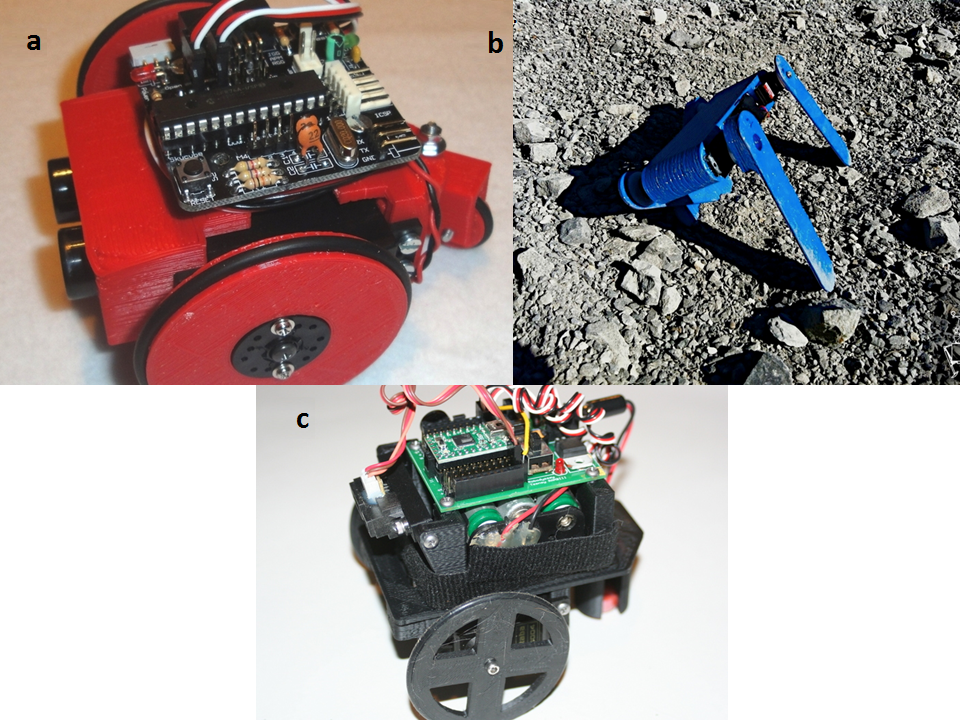
\includegraphics[width=1\textwidth]{./Figures/thingiverse.png}
		\rule{35em}{0.5pt}
	\caption[Robots en Thingiverse]{Robots que han sido subidos a la plataforma Thingiverse para que usuarios puedan descargar los modelos y construirlos. \textbf{a.} MiniSkybot, \textbf{b.}SlinkyBOT Lunar mini rover y \textbf{c.} Econo1Bot for the RAMB motherboards.}
	\label{fig:thingiverse}
\end{figure}

%-----------------------------------
%	SECTION 3
%-----------------------------------
\section{Necesidades de mercado}

De los robots estudiados destaca en sus prestaciones el e-puck, pero este tiene dos grandes problemas para ser usado por gente que no es especialista en robots. Uno es que tiene demasiado hardware, lo que tiende a confundir y aumentar costos. Dos, que para su comunicación inalámbrica hace uso de Bluetooth, protocolo que no soporta las redes Mesh para hacer de manera simple el control de muchos dispositivos en una red. Por otro lado el robot Kilobot es extremadamente simple, no permite mucha modificación y este con 3pi no tienen sistema de comunicación inalámbrica.

Hace falta un robot que no sobrepase los 200 USD, capaz de controlarse en forma inalámbrica, simple de construir y fácil de usar. Se requiere hacer uso de tecnologías como impresoras 3D y diseño Open Hardware para los robot que formen el enjambre. El tener un diseño compatible con las impresoras 3D facilita enormemente la difusión y distribución del proyecto, ya que cualquier persona con acceso a una impresora 3D puede replicar el robot. Y para hacer más simple el proceso de réplica y fomentar las mejoras en el proyecto, se requiere que tanto el hardware como el software sean Open, esto significa que cualquier persona puede acceder a los archivos de diseño del robot, copiarlos, redistribuirlo y modificarlo para que se adapte a sus necesidades. El nombre del robot será MODI que viene de las siglas del inglés Modular Intelligence. MODI quiere satisfacer el nicho de mercado donde se necesitan robots simples y de bajo precio, como se ve en la Figura \ref{fig:nicho}.

\begin{figure}[htbp]
	\centering
		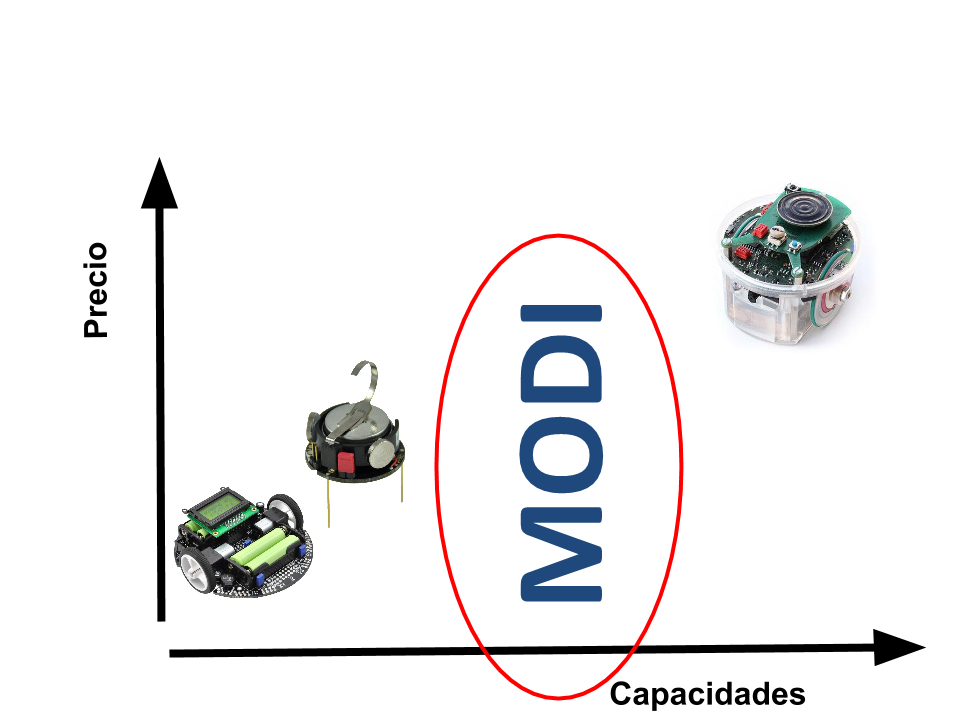
\includegraphics[width=0.7\textwidth]{./Figures/nicho.png}
		\rule{35em}{0.5pt}
	\caption[Nicho de mercado]{Nicho de mercado donde puede ingresar la plataforma robótica que se diseñó. Su nombre es MODI por las siglas en inglés de Modular Intelligence.}
	\label{fig:nicho}
\end{figure}




\chapter{Diseño y fabricación digital} 

\label{Chapter4} 

\lhead{Capítulo 4. \emph{Diseño y fabricación}} %

%----------------------------------------------------------------------------------------
%	SECTION 1
%----------------------------------------------------------------------------------------
\begin{figure}[htbp]
	\centering
		\includegraphics[width=0.8\textwidth]{./Figures/FabDig.JPG}
	%	\rule{35em}{0.5pt}
	%\caption[Robot MODI]{robot MODI (sigla para Modular Intelligence)}
	\label{fig:FabDig}
\end{figure}

Como se expuso en el capítulo anterior, actualmente existen varias alternativas de robots para comprar y construir un enjambre de robots. El problema es que o su precio es demasiado elevado o simplemente no son adaptables al tipo de investigación que se quiere realizar. Nuestro objetivo es tener un robot económico, fácil de reproducir y fabricable en la universidad para construir un enjambre de robots que permita hacer investigación y desarrollos en esta área.


\section{Requerimientos de desarrollo}

Para satisfacer los objetivos de diseño de MODI se pretende cumplir con los siguientes requerimientos:
\newpage 
\textbf{Requerimientos de desarrollo}

\begin{enumerate}
\item \textbf{Simple de fabricar}: Mientras más simple de fabricar sea MODI, más fácil va a ser reproducirlo para tener muchos robots en el enjambre. Esto también permite mantener los costos de fabricación bajos. 
\item \textbf{Open Source, Open Hardware}: Si se liberan tanto el código fuente del robot como la información detallada del Hardware es más fácil que otros laboratorios puedan replicar este trabajo y a su vez mejorarlo. Una de las ventajas de seguir la filosofía \textit{Open} en el desarrollo es que los que hagan uso de nuestro Hardware o Software están comprometidos a compartir sus mejoras.
\item \textbf{Fabricable en un Fab Lab}: Actualmente existen cerca de 263 Fab Labs en el mundo, así que tener un diseño compatible con las maquinarias que utilizan los Fab Labs ayuda a poder difundir este trabajo. Los componentes que no puedan ser fabricados deben ser de fácil acceso.
\item \textbf{Minimizar la cantidad de componentes mecánicos extras necesarios}: La base del diseño mecánico del robot debe ser el Chasis de éste, pieza encargada de unir todos los componentes. No debe necesitar tornillos ni silicona para ensamblarlo.
\item \textbf{Carga Autónoma}: El robot debe contar con un sistema que facilite la carga de energía autónoma para poder realizar experimentos de larga duración sin intervención humana. Debe permitir diferentes tipos de carga como inductiva o con panel solar.
\item \textbf{Sistema de tracking}: Es necesario poder obtener la posición y orientación de cada uno de los robots. Por lo que el setup para todos los robots debe contar con una cámara que permita con procesamiento de imágenes obtener esta información.
\item \textbf{Control individual del color de cada MODI}: Para poder observar de manera rápida el estado de cada robot es necesario que cada uno cuente con un LED RGB.
\item \textbf{Movimiento simple de cada robot de forma independiente}: Cada robot debe ser capaz de recibir y ejecutar órdenes simples de movimiento en el plano.
\item \textbf{Comunicación inalámbrica}: Cada robot debe ser capaz de enviar y recibir informacion de manera inalámbrica con un servidor central. Debe tener la posibilidad de construir redes entre los robots también.
\end{enumerate}


La función principal de MODI es ser una plataforma móvil de fácil acceso. Existe un repositorio en GitHub  \footnote{https://github.com/FabLabUChile/modi} donde se tienen los códigos actualizados para controlar y construir robots MODI. Todo esto para poder cumplir con el \textbf{requerimiento 2}. Una lista con componentes extras para comprar se encuentra en la Figura \ref{fig:BOM}. Esta lista de materiales cumple con el \textbf{requerimiento 4}. 

El Robot MODI es Open Hardware, por lo mismo sus archivos se encuentran en el repositorio GitHub nombrado anteriormente. Todas las piezas que componene al robot son de libre distribución y uso, además pueden modificarse a gusto. La estructura de archivos se puede ver en la Figura \ref{fig:tree}, donde están los archivos del Hardware, Software y los que generar este documento Latex.
\begin{figure}[htbp]
	\centering
		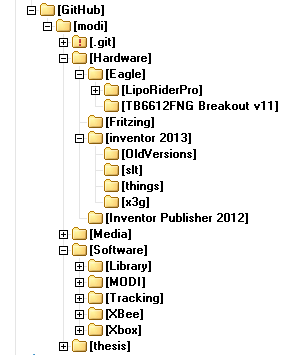
\includegraphics[width=0.8\textwidth]{./Figures/MODI/tree.png}
		\rule{35em}{0.5pt}
	\caption[Estructura de archivos]{Estructura de archivos necesarios para construir robots MODIs y programarlos.}
	\label{fig:tree}
\end{figure}



%-----------------------------------
%	SECTION 2
%-----------------------------------

\section{Fabricación Digital}

La Fabricación Digital es una técnica que permite una traducción directa del mundo digital al mundo físico. Gracias a esta es posible diseñar y contruir con presición objetos y formas cuya geometrías dificilmente podrían ser logrados en una producción artesanal o industrial. Es por esto que es una técnica perfecta para el desarrollo del proyecto MODI. Construir un robot implica el diseño en computador de varios componentes. Estos pueden ser circuitos electrónicos (PCB), software de control y piezas mecánicas. Uno de los requerimientos principales del desarrollo es que sea simple de fabricar, es por esto que en el resultado final se reflejan las horas de diseño. Las herramientas que se necesitan son software CAD para el modelado y diversas maquinas que construyan con presición los modelos diseñados en el software CAD. Algunas maquinas son: impresora 3D, Router CNC y cortadora LASER.




%-----------------------------------
%	SUBSECTION 3
%-----------------------------------
\subsection{Software CAD}

CAD viene de sus siglas del inglés, Computer-aided design, y se refiere a un diseño asistido por herramientas computacionales. Profesionales como ingenieros, arquitectos y del área del diseño por lo general son los que hacen más uso de estas herramientas.

Los software CAD se pueden dividir en programas de dibujo para dos dimensiones (2D) y modeladores en tres dimensiones (3D). Las herramientas de dibujo en 2D se basan en entidades geométricas vectoriales como puntos, líneas, arcos y polígonos, con las que se puede operar a través de una interfaz gráfica.

Durante el transcurso del proyecto se trabajó con varios softwares CAD. El primero fué SketchUp 8 de Google, que permite fácilmente hacer bocetos de lugares y cuenta con una importante biblioteca de modelos para incluir en el diseño. Rápidamente se pudo hacer un scketch utilizando modelos descargados de Internet, ver Figura~\ref{fig:setup}. Para el diseño del chasis del robot se utilizó SolidWorks 2012 y luego por ser más simple de usar, Inventor 2013 de Autodesk. Ambos softwares permiten generar modelos en 3D para luego exportar el diseño al formato STL que es estándar para prototipar en plástico. 




%-----------------------------------
%	SUBSECTION 2
%-----------------------------------
\subsection{Impresoras 3D}
Cuando se quiere pasar una idea al mundo real es necesario un proceso de fabricación. Dependiendo de la cantidad de herramientas que se tenga es más o menos fácil la tarea. Desde el comienzo hasta hace un par de años, quienes se dedican a construir robots, debían construir de manera \textit{artesanal} donde es imposible que las piezas queden todas iguales y el tiempo empleado era bastante. Hoy en día existe una gran alternativa, la Fabricación Digital, que surge como un nuevo paradigma de construcción y una herramienta clave que son las impresoras 3D. Las impresoras 3D, existen desde los 80' y hasta hace algunos años por su precio y tamaño eran de difícil acceso. Utilizan distintas tecnologías; las que se usaron en el proceso de este trabajo son las FDM, sigla del inglés "Fused deposition modeling" donde un cabezal extrusor de plástico se mueve en el plano xy depositando capa por capa de material mientras avanza en el eje z, ver Figura \ref{fig:3Dprint}. En este trabajo primero se utilizó la 3D Touch Dual de la empresa Bit from Bytes, ver Figura \ref{fig:impresoras} a, que permite hacer modelos de hasta 185 x 273 x 200[mm], con una buena resolución de 0.125[mm]\footnote{teambastech.com/Store/index.php?route=product/product\&product\_id=205} cada capa en eje z. Luego por facilidad de uso y menor tiempo de impresión se usa una impresora MakerBot Replicator 1, ver Figura \ref{fig:impresoras} c. También existen otros tipos de máquinas que permiten hacer diseños en 2D, éstas son las cortadoras LASER. La primera versión de MODI fue construida usando planchas de madera MDF y acrílico, cortados en LASER, ver figura \ref{fig:analgTodigital} a. Hacer uso de estas máquinas permite cumplir con los \textbf{requerimientos 1 y 3}.

\begin{figure}[htbp]
	\centering
		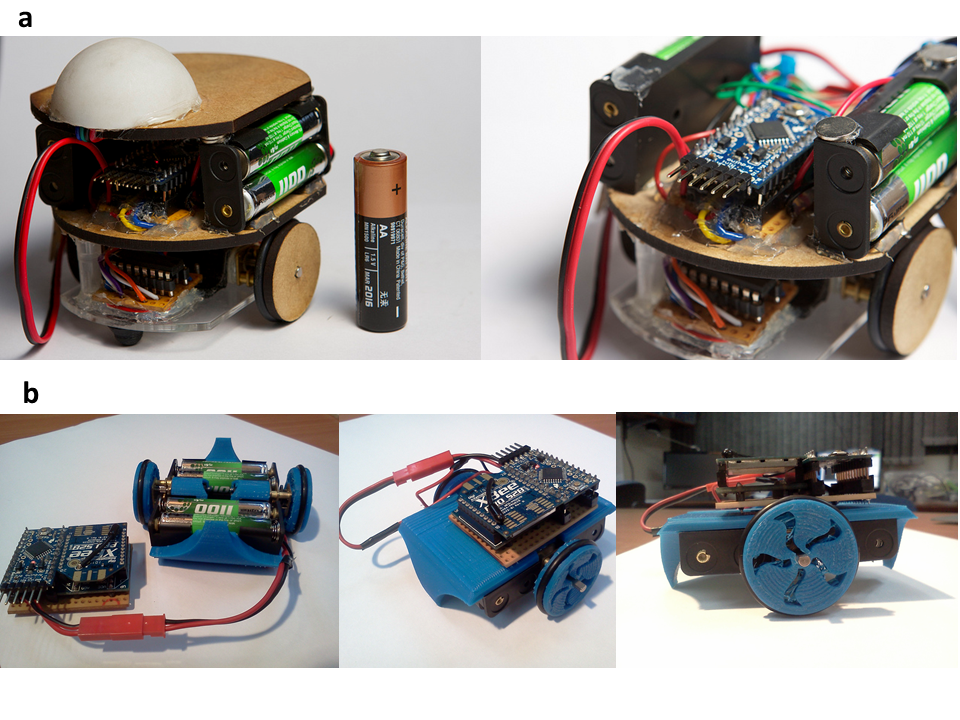
\includegraphics[width=0.8\textwidth]{./Pictures/modi_analogToDigital.png}
		\rule{35em}{0.5pt}
	\caption[Comparación de construcción análoga y digital]{\textbf{a.} Primera versión MODI construida con MDF y bastante silicona. Esta versión presentaba el problema de involucrar demasiadas partes que debían ser hechas por una persona. \textbf{b.} MODI usando técnica de \emph{ Fabricación Digital }con chasis de plástico construido con una MakerBot Replicator 1}
	\label{fig:analgTodigital}
\end{figure}

\begin{figure}[htbp]
	\centering
		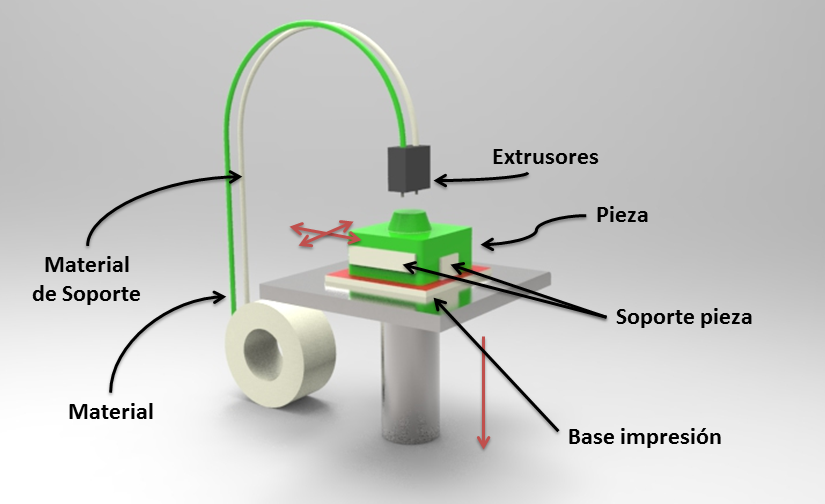
\includegraphics[width=\textwidth]{./Figures/3Dprint.png}
		\rule{35em}{0.5pt}
	\caption[Modelo funcionamiento Impresora 3D]{Modelo de funcionamiento impresoras 3D FDM. Tiene dos materiales, uno para construir la pieza y otro que funciona como soporte estructural para la impresión. Además existe una base que se calienta para sujetar la pieza mientras se construye. Puede moverse tanto la base como el extrusor para generar el modelo.}
	\label{fig:3Dprint}
\end{figure}	



\begin{figure}[htbp]
	\centering
		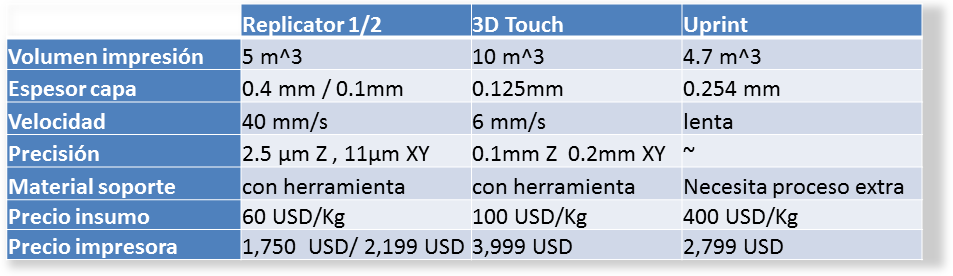
\includegraphics[width=\textwidth]{./Figures/tabla_impresoras.png}
		\rule{35em}{0.5pt}
	\caption[Tabla comparativa de Impresoras 3D]{Tabla comparativa de las características más importantes de impresoras 3D, Replicator 1, 3D Touch y Uprint}
	\label{fig:TablaImpresoras}
\end{figure}


\begin{figure}[htbp]
	\centering
		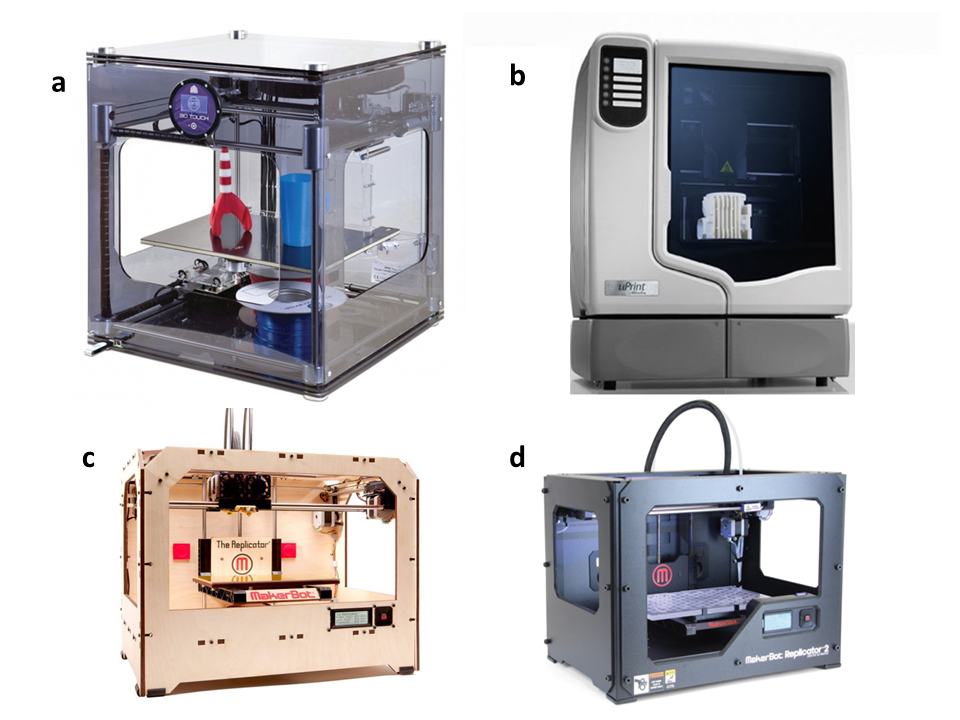
\includegraphics[width=\textwidth]{./Figures/impresoras.png}
		\rule{35em}{0.5pt}
	\caption[Impresoras 3D]{\textbf{a.} 3D Touch Dual de la empresa Bit from Bytes, \textbf{b.} Uprint SE de Stratasys, \textbf{c.} Replicator 1 de Makerbot, impresora 3D FDM utilizada para prototipar chasis y ruedas de robot MODI, \textbf{d.} Replicator 2 de MAkerbot, tiene mejor resolución que la versión 1.}
	\label{fig:impresoras}
\end{figure}	

%\FloatBarrier

Aunque han bajado los precios de las máquinas para prototipado rápido, aún no están al alcance de todas las personas. Es por esto que existen los Fab Labs (acrónimo del inglés Fabrication Laboratory), que es un espacio de producción de objetos físicos a escala personal o local que agrupa máquinas controladas por ordenadores. Su particularidad reside en su tamaño y en su fuerte vinculación con la sociedad. Los Fab Labs están por todo el mundo, Figura \ref{fig:Fablabs}. MODI fue concebido como un proyecto del Fab Lab de la Universidad de Chile y por esto es posible reproducirlo en cualquier Fab Lab. En Chile, además del Fab Lab de la Universidad de Chile están: Design LAB UAI, Fab Lab Santiago y Stgo MakerSpace. 

\begin{figure}[htbp]
	\centering
		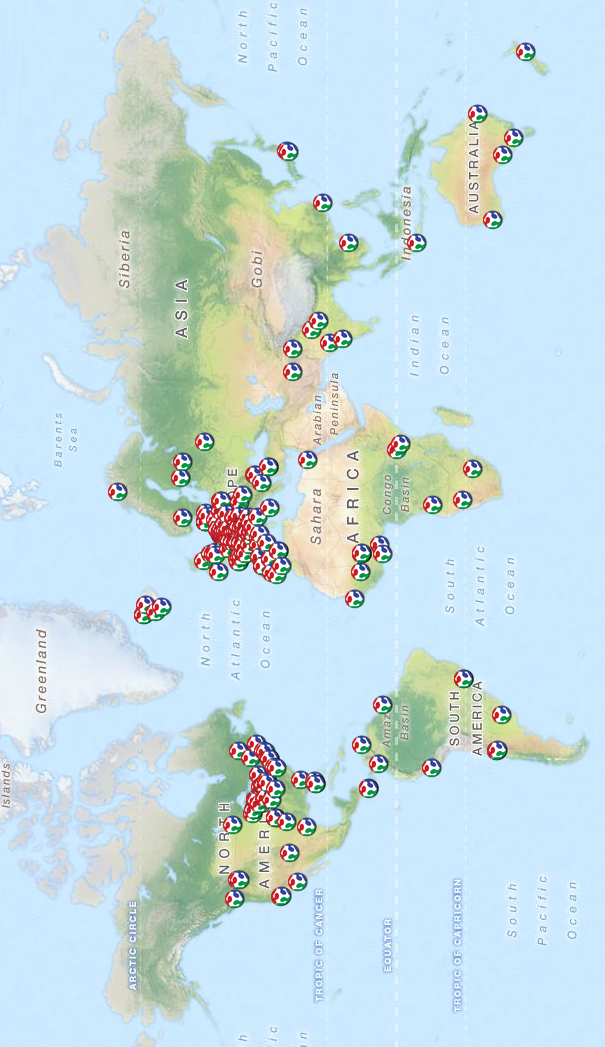
\includegraphics[width=0.9\textwidth]{./Figures/map.png}
		\rule{35em}{0.5pt}
	\caption[Mapa Fab Labs en el mundo.]{Mapa actual de lugares en el mundo que cuentan con un Fab Lab, actualmente en el sitio http://wiki.fablab.is/wiki/Portal:Labs se registran 263. En Chile a la fecha existen 3. Imagen tomada de fablabamersfoort.nl/fablabs/}
	\label{fig:Fablabs}
\end{figure}	

Para la construcción del Robot MODI es necesario contar con una impresora 3D del tipo FDM, y una máquina que permita construir PCB electrónicas de una sola capa.



 
% Chapter Template

\chapter{MODI} % Main chapter title

\label{Chapter5} % Change X to a consecutive number; for referencing this chapter elsewhere, use \ref{ChapterX}

\lhead{Capítulo 5. \emph{MODI}} % Change X to a consecutive number; this is for the header on each page - perhaps a shortened title

%----------------------------------------------------------------------------------------
%	SECTION 1
%----------------------------------------------------------------------------------------
\begin{figure}[htbp]
	\centering
		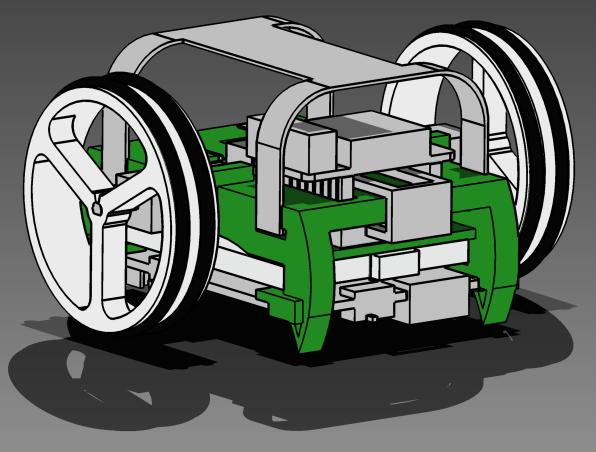
\includegraphics[width=0.8\textwidth]{./Figures/MODI/render.png}
	%	\rule{35em}{0.5pt}
	%\caption[Robot MODI]{robot MODI (sigla para Modular Intelligence)}
	\label{fig:MODI}
\end{figure}

Como se expuso en el capítulo anterior, actualmente existen varias alternativas de robots para comprar y construir un enjambre de robots. El problema es que o su precio es demasiado elevado o simplemente no son adaptables al tipo de investigación que se quiere realizar. Nuestro objetivo es tener un robot económico, fácil de reproducir y fabricable en la universidad para construir un enjambre de robots que permita hacer investigación y desarrollos en esta área.

\section{Desarrollo de MODI}

En este trabajo para el desarrollo solamente del robot MODI se tomó un año, periodo durante el cual se hicieron muchos prototipos del chasis plastico que contiene la electrónica y también la electrónica tuvo cambios que fueron puliendo el diseño. 
\subsection{Electrónica de MODI}
Principalmente se tuvo que reducir lo más posible la cantidad y tamaño de los componentes, siempre haciendo uso de componentes fácil de conseguir en el mercado y que fueran de bajo costo. Otro aspecto importante a considerar en la elección de la electrónica fue el sistema de energía, que finalmente se optó por utilizar baterías del tipo Litio Polimero por su alta densidad de carga y la posibilidad de regargala con la misma tarjeta electrónica que controla el robot. Fundamental fue el uso de la paltaforma Arduino, que es un microcontrolador de fácil uso y ampliamente difundido en el mundo.
\subsection{Chasis de MODI}
El diseño del chasis fue sometido a varios cambios, primero para adaptarse a la electrónica escogida que tuvo varios cambios y segundo, este chasis debía ser pequeño y tener solo lo necesario. Es por esto que fue clave modelar cada uno de los componentes electrónicos para poder diseñar un chasis con un ajuste preciso a estos. Otro aspecto importante fue eliminar completamente las uniones hechas con silicona y el uso de pernos, para al final llegar a un diseño en que solo se utilizan piezas plasticas que encajan entre si.

\section{Diseño de Chasis MODI}
Luego de varias iteraciones (ver Figura \ref{fig:Historia})se logró el modelo final, ver Figura \ref{fig:compRender} b, que tiene cuatro piezas hechas en plástico PLA como se puede ver en la Figura \ref{fig:DiagramaVersionFinal}. En la Figura \ref{fig:modi real} hay unas fotos de siete robots MODI versión final y un robot MODI versión anterior. En la Figura \ref{fig:MODI Detalle} se puede ver en detalle un robot MODI.

\begin{figure}[htbp]
	\centering
		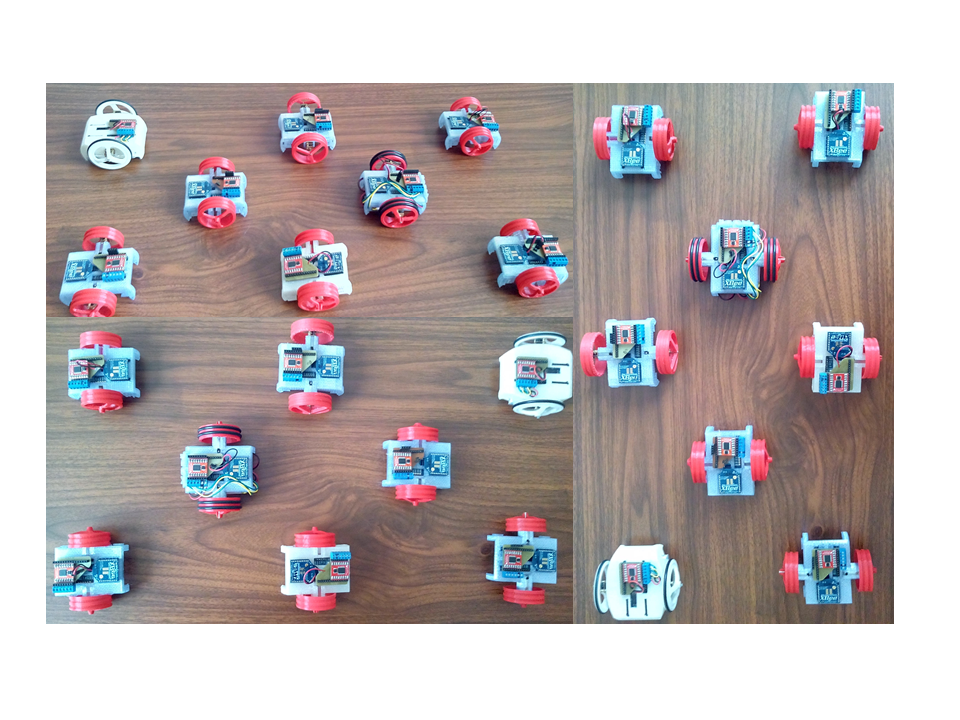
\includegraphics[width=\textwidth]{./Figures/MODI/modi_real.png}
		\rule{35em}{0.5pt}
	\caption[MODI Swarm]{Fotos de enjambre de MODI, formado por siete robots MODI versión final y un robot MODI versión anterior. Robots MODI versión final ensamblados por Andres Ulloa.}
	\label{fig:modi real}
\end{figure}


\begin{figure}[htbp]
	\centering
		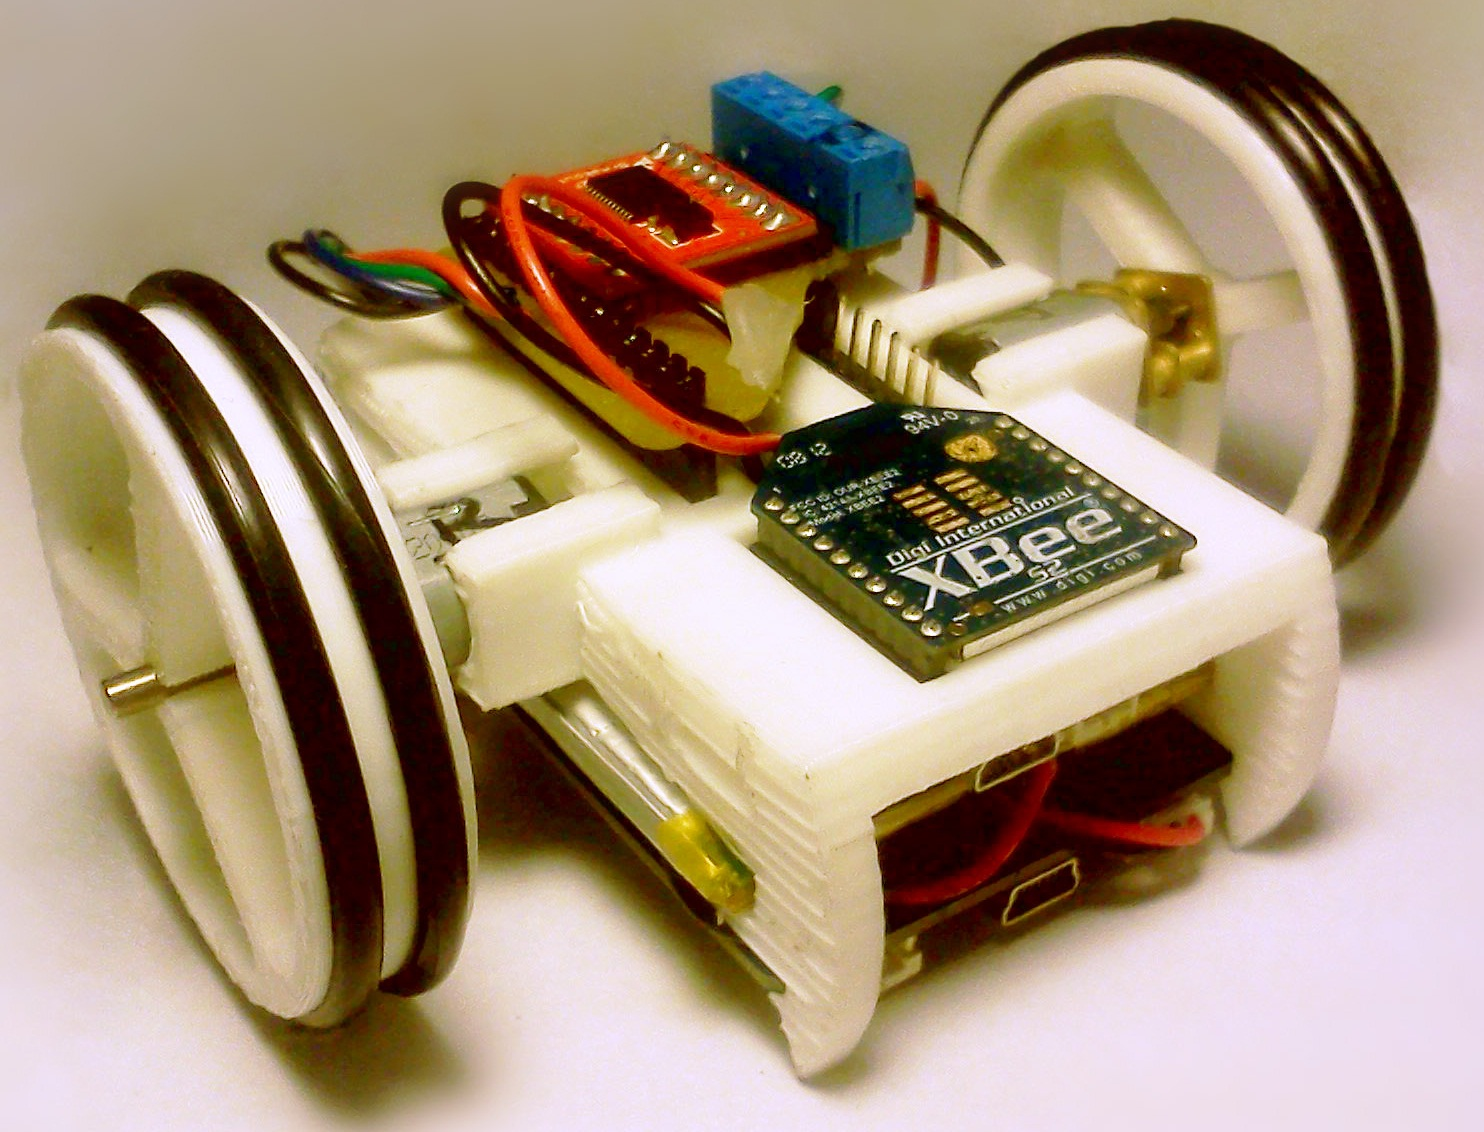
\includegraphics[width=\textwidth]{./Pictures/modi_photo.jpg}
		\rule{35em}{0.5pt}
	\caption[MODI Detalle]{Fotografía de robot MODI.}
	\label{fig:MODI Detalle}
\end{figure}

Las piezas del robot fueron diseñadas para ser construidas por una máquina de prototipado rápido del tipo FDM, como una Reprap o MakerBot Replicator 2. Se debe tener en cuenta la tolerancia mecánica de las piezas. En especial hay dos piezas: la rueda y el chasis, que se unen al motor. Esta unión debe quedar con un ajuste mecánico Forzado Medio \footnote{http://campuscurico.utalca.cl/\~ fespinos/Ajustes\%20y\%20tolerancias\%20mecanicas.pdf}, para que estas uniones queden fijas y las ruedas estén en el eje correspondiente.

Está formado por cuatro partes:

\begin{enumerate}
\item Chasis, que es la pieza que une a todos los componentes y cumple con el \textbf{Requerimiento 4}. Ver Figura \ref{fig:Render Piezas 3D} a.
\item Ruedas, permiten el desplazamiento y poseen dos canales para poner o-ring y así aumentar el roce con la supercifie. Ver Figura \ref{fig:Render Piezas 3D} d.
\item Accesorio, tiene un sistema de anclaje al chasis que permite tener distintas carcasas y sensores. Ver Figura \ref{fig:Render Piezas 3D} b.
\item Logo,  sujeta parte de la electrónica contenida en el Chasis y dos LEDs RGB. Ver Figura \ref{fig:Render Piezas 3D} c.
\end{enumerate}

Cada una de estas piezas puede ser vista en la Figura \ref{fig:Render Piezas 3D}.

Usando una Replicator 1 de MakerBot, la pieza que más demora en construirse es el Chasis, que son 108 minutos. Cada Rueda demora 20 minutos, el accesorio 58 minutos y el logo 25 minutos. En la la Figura \ref{fig:tabla impresion} hay una tabla que resume esto.

\begin{figure}[htbp]
	\centering
		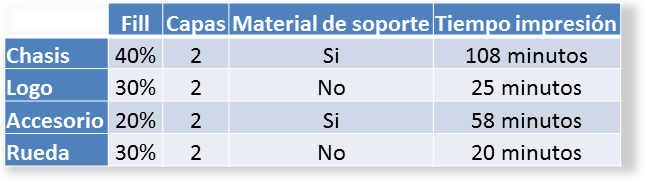
\includegraphics[width=0.8\textwidth]{./Figures/MODI/tablaimpresion.png}
		\rule{35em}{0.5pt}
	\caption[Tabla impresion]{Tabla que resume los tiempos y configuración de impresión de las piezas de MODI en una MakerBot Replicator 1.}
	\label{fig:tabla impresion}
\end{figure}

\begin{figure}[htbp]
	\centering
		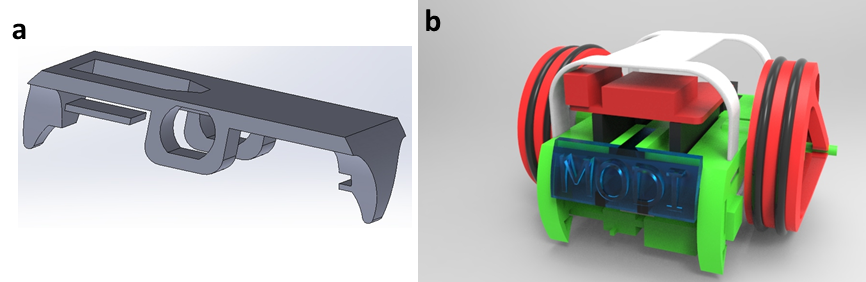
\includegraphics[width=\textwidth]{./Figures/MODI/compRender.png}
		\rule{35em}{0.5pt}
	\caption[Comparación entre el primer render realizado y el último]{\textbf{ a.} Primer Chasis de MODI, realizado con SolidWorks 2012. Esta versión sirve sólo como prueba de concepto ya que no tiene espacio para las conexiones eléctricas necesarias.\textbf{ b.} Última versión de MODI a la fecha, el diseño se realizó en Inventor 2013 y el render se obtuvo con KeyShot 4.}
	\label{fig:compRender}
\end{figure}	

\begin{figure}[htbp]
	\centering
		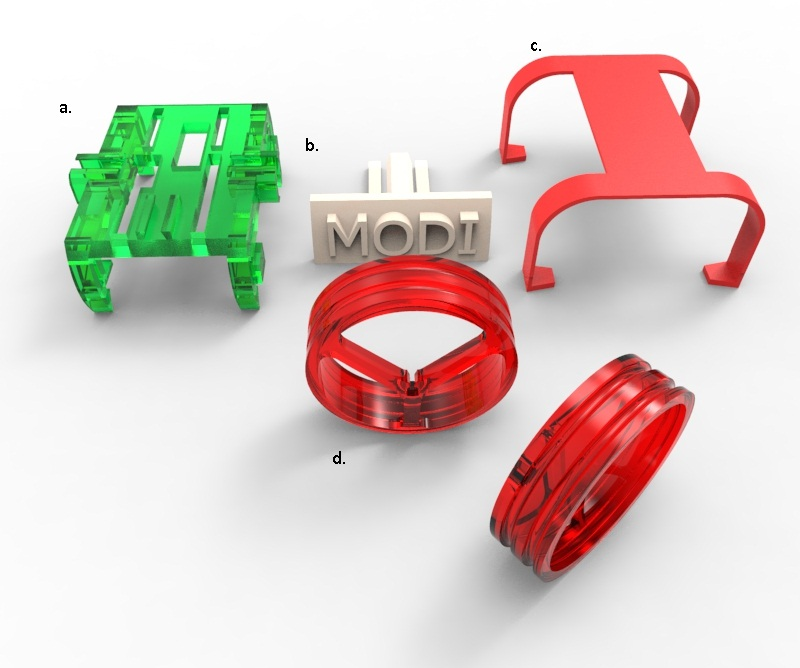
\includegraphics[width=\textwidth]{./Figures/MODI/piezas.jpg}
		\rule{35em}{0.5pt}
	\caption[Piezas 3D]{Las cinco piezas que componen el hardware mecánico de MODI, estas son: a) el chasis, d) las dos ruedas, c) el accesorio y b)logo. Las dimensiones del robot MODI ensamblado son 96[mm] de diámetro y 50 [mm] de alto.}
	\label{fig:Render Piezas 3D}
\end{figure}

\begin{figure}[htbp]
	\centering
		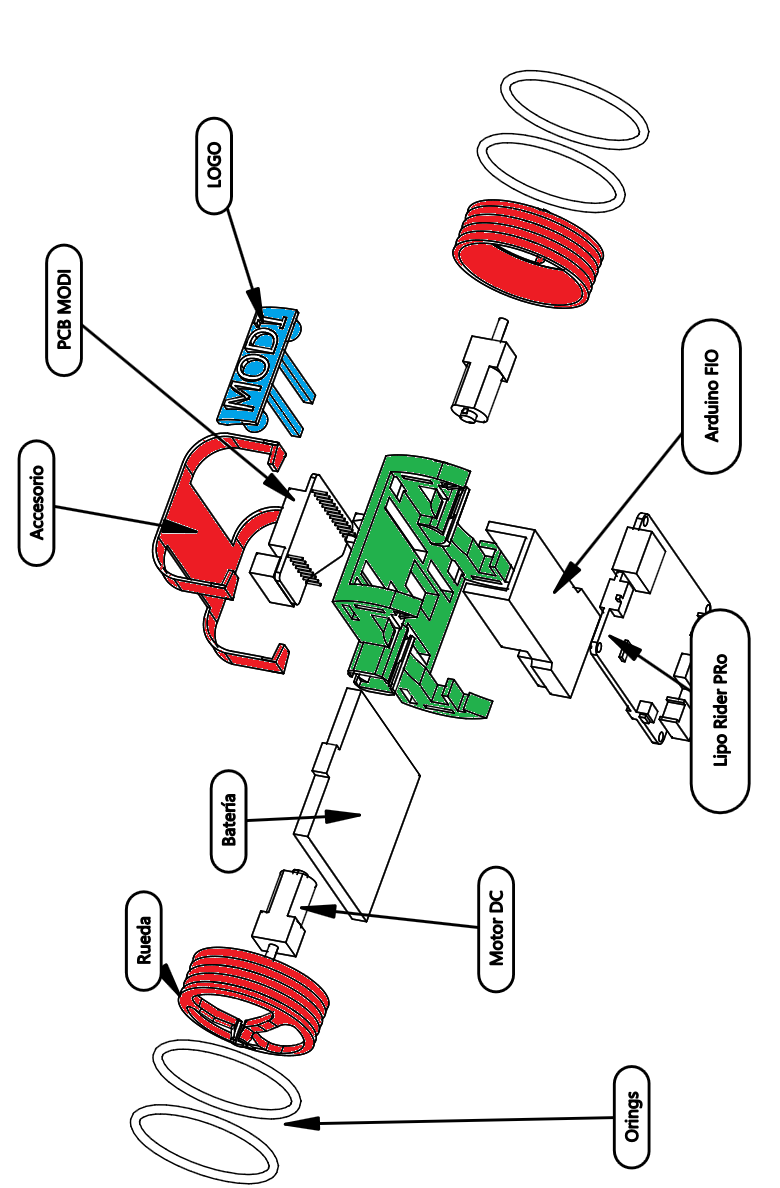
\includegraphics[width=\textwidth]{./Figures/MODI/ensamble.png}
		\rule{35em}{0.5pt}
	\caption[Diagrama MODI versión final]{Diagrama de todos los componentes que forman parte de MODI, este diagrama sirve de guía para poder ensamblarlo. Las piezas Logo y Accesorio permite personalizar a MODI y también incorporar sensores extras.}
	\label{fig:DiagramaVersionFinal}
\end{figure}	

\FloatBarrier
%-----------------------------------
%	SUBSECTION 5
%-----------------------------------
\section{Diseño de PCB MODI}

En los primeros prototipos un problema que se repetía constantemente fueron las conexiones entre los sistemas que componen al robot. Son 15 conexiones que unen distintos componentes, Figura \ref{fig:Diagrama cables}. Por esto se requiere un PCB que permita reducir al mínimo el espacio necesario para energizar y comunicar los componentes. El requerimiento principal es poder fabricarlo con una fresa CNC como la Roland Modela MDX-20 (disponible en el FABLAB UCHILE), por lo que para facilitar el proceso de construcción es necesario diseñar un PCB de una sola capa. Se utilizó Eagle como software para el diseño del diagrama eléctrico y PCB, el resultado se puede ver en la Figura \ref{fig:pcb}.


\begin{figure}[htbp]
	\centering
		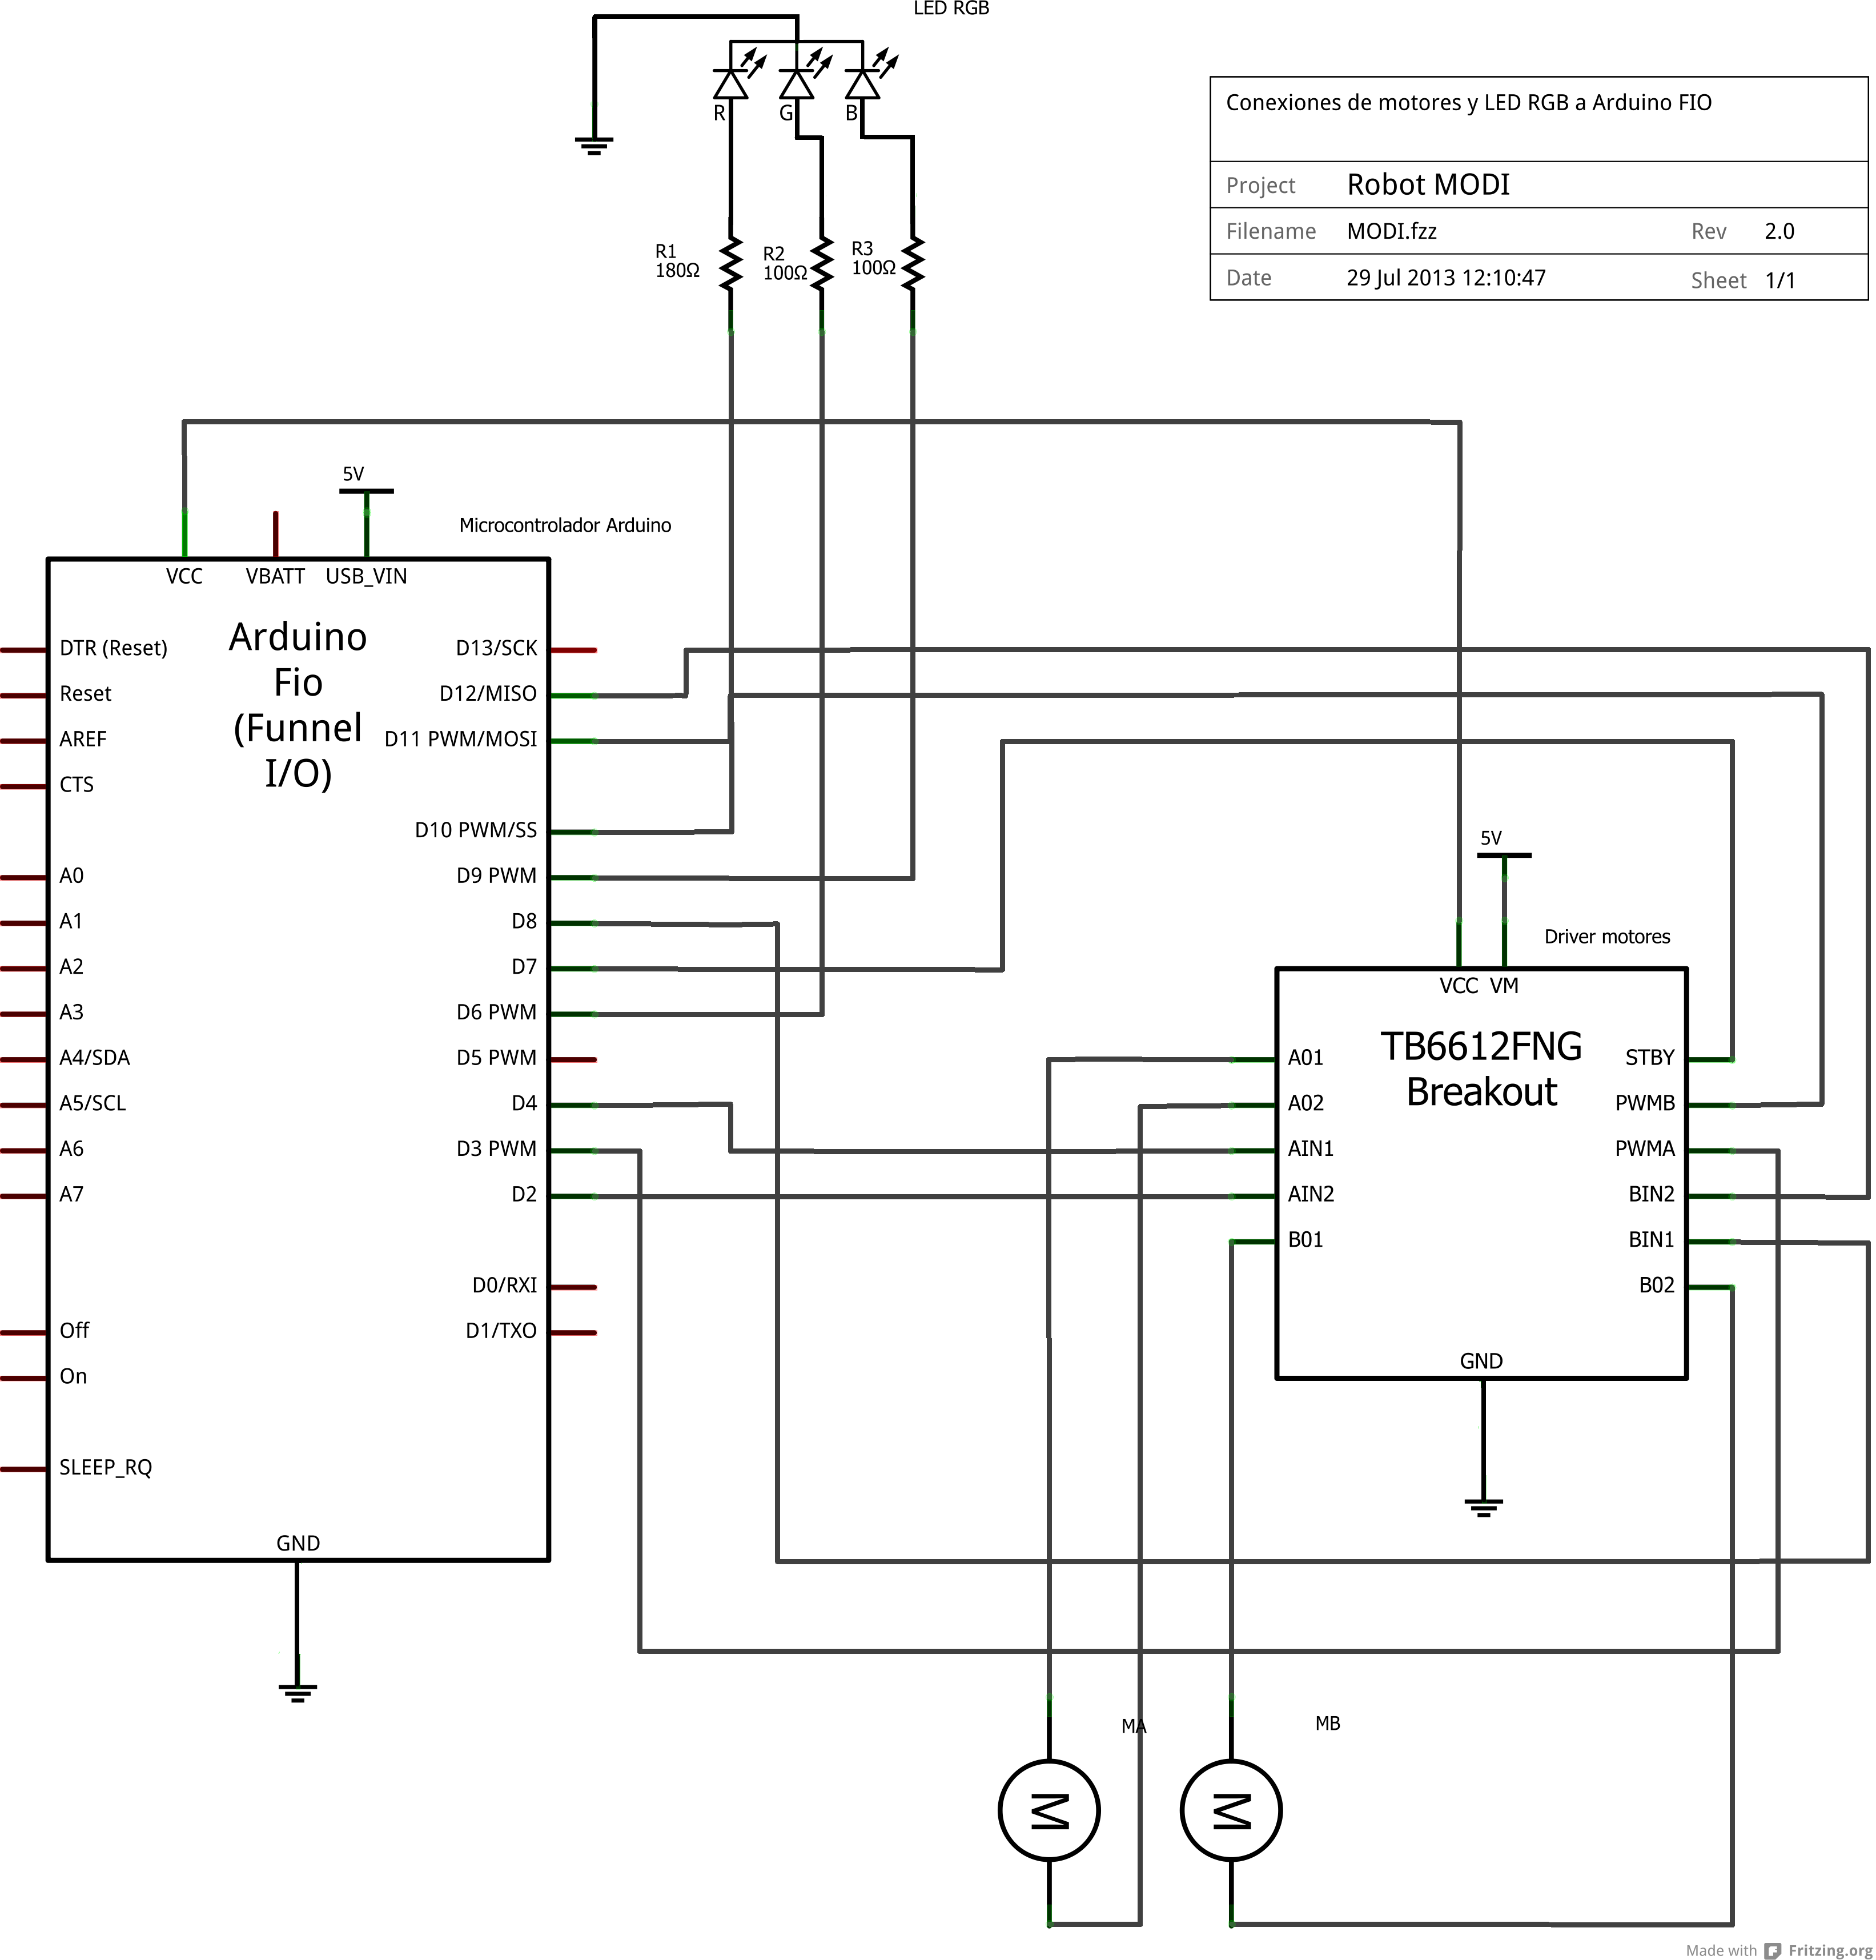
\includegraphics[width=\textwidth]{./Figures/modi/MODI_schem.png}
		\rule{35em}{0.5pt}
	\caption[Diagrama eléctrico de conexiones en PCB MODI]{Diagrama de conexiones eléctricas en PCB diseñada para MODI. Está realizado en Fritzing.2013.07.27.pc.}
	\label{fig:Diagrama cables}
\end{figure}	

\begin{figure}[htbp]
	\centering
		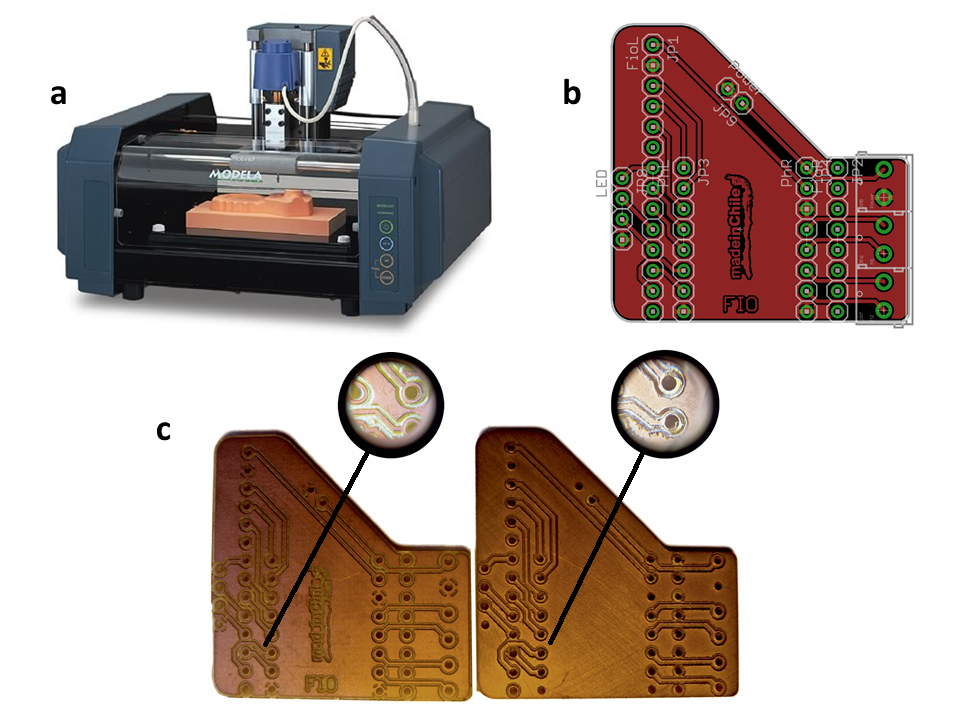
\includegraphics[width=0.9\textwidth]{./Figures/modi/pcb.png}
		\rule{35em}{0.5pt}
	\caption[Fabricación de PCB]{\textbf{a.} Roland Modelo MDX-20 usada para hacer PCB y modelos 3D \textbf{b.} MODIBoard es una PCB diseñada para poder conectar de forma simple los diversos componentes electrónicos. Conecta: Arduino Fio, Lipo Rider Pro, Motor Driver, LED RGB y Motores, \textbf{c. }PCB fresada en dos máquinas diferentes. Se puede apreciar en el detalle aumentado 60x, la importancia de contar con una buena resolución de fresado como en la imagen de la izquierda donde incluso se pudo hacer el logo. En especial es necesario tener un buen pad para facilitar el soldado.}
	\label{fig:pcb}
\end{figure}

En la Figura \ref{fig:ComponentesPCB} hay una fotografía con todos los componentes necesarios para ensamblar una PCB MODI, para controlar motores con un Arduino FIO.

\begin{figure}[htbp]
	\centering
		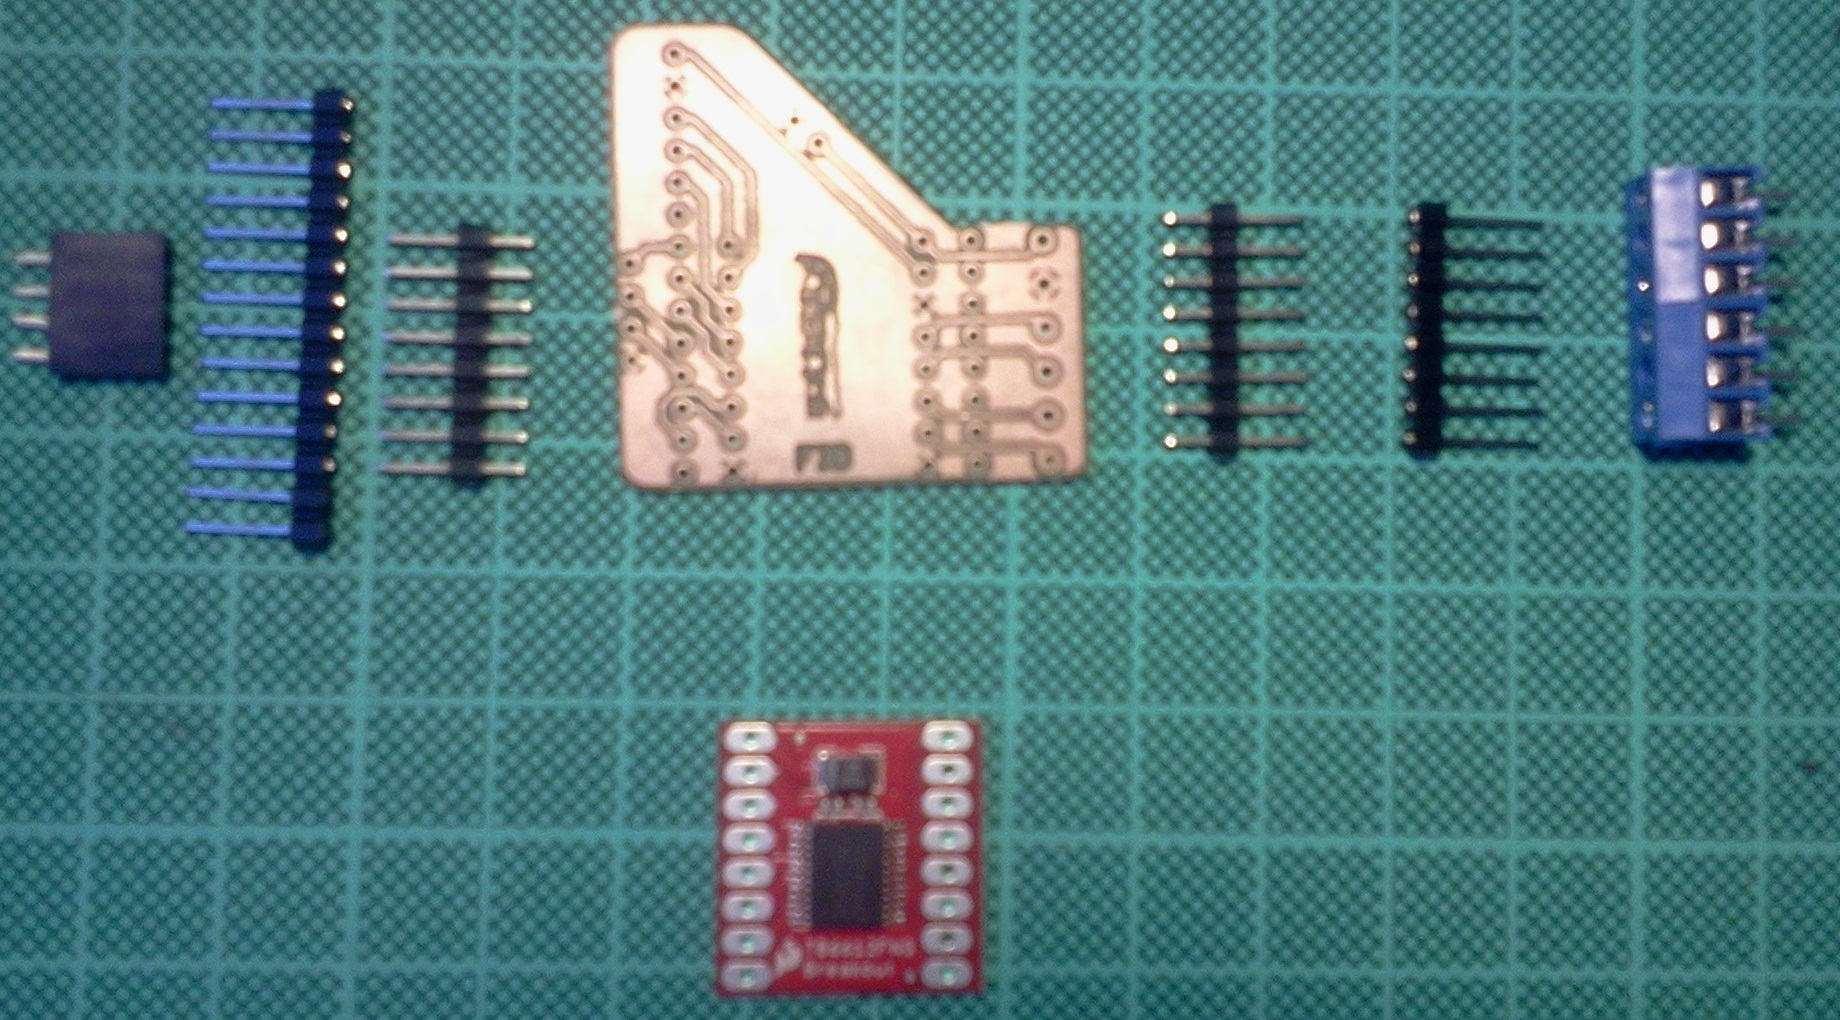
\includegraphics[width=\textwidth]{./Pictures/soldado.jpg}
		\rule{35em}{0.5pt}
	\caption[Componentes PCB MODI antes de soldar]{Fotografía de todos los componentes para ensamblar una PCB MODI.}
	\label{fig:ComponentesPCB}
\end{figure}	


%-----------------------------------
%	SECTION 2
%-----------------------------------

\section{Componentes electrónicos}

\begin{figure}[htbp]
	\centering
		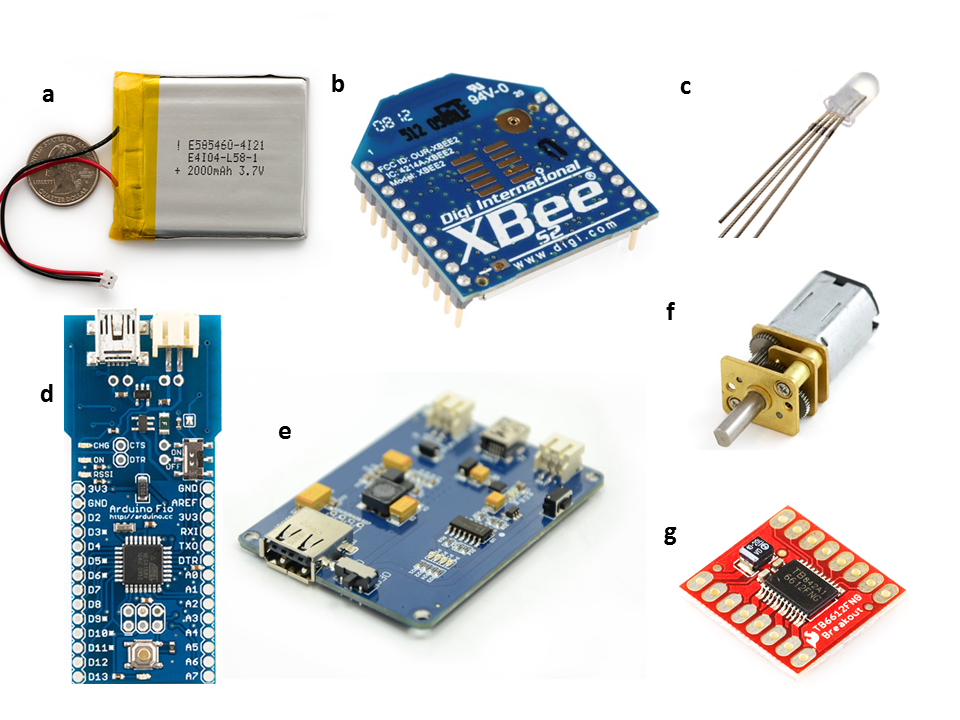
\includegraphics[width=\textwidth]{./Figures/MODI/compElo.png}
		\rule{35em}{0.5pt}
	\caption[Componentes Electrónicos]{Todos los componentes electrónicos que forman MODI \textbf{ a.} Batería LIPO 2,000 mAh, \textbf{b.} XBee, \textbf{c.} LED Rgb difuso, de esta manera se obtiene un ángulo de visión mucho más amplio, \textbf{d.} Arduino Fio, \textbf{e.} Lipo Rider Pro,\textbf{ f.} Motor DC 30:1 \textbf{g.} Motor Driver 1A Dual TB6612FNG.}
	\label{fig:compELO}
\end{figure}

MODI está compuesto por varios componentes electrónicos que implementan tecnologías nuevas. De forma sencilla el usuario puede hacer uso de todas estas, que por ser Open Source tienen una amplia documentación. Su uso en colegios, talleres y universidades, por ser de bajo costo, y sin partes externas extremadamente frágiles, es una excelente herramienta para iniciar a alumnos en temas como la Programación, Robótica, Comunicación Inalámbrica y Visión Artificial, entre otros, sin los miedos asociados a utilizar un equipo costoso y delicado.

El robot MODI es pequeño y de fácil construcción con las herramientas de Fabricación Digital que se pueden encontrar en un FabLab. Tiene un pequeño microcontrolador \textbf{Arduino} que controla dos motores, y un \textbf{XBee} para la comunicación inalámbrica con un computador central que usando cualquier lenguaje de programación con comunicación serial puede controlar uno o más robots. La posición de cada robot se obtiene con tags \textbf{Fiduciales}, que permiten por medio de una cámara cenital saber la coordenada y rotación de cada uno, de esta forma se ahorra en costosos sistemas de tracking 2D. En esta primera aplicación es necesario contar con autonomía energética por lo que se incluye una batería lipo de 2000[mAh] junto a un módulo que carga la batería y eleva el voltaje de salida a 5[v]. Este módulo de carga, \textbf{Lipo Rider Pro}, tiene además la ventaja de permitir distintos tipos de carga, como una celda de carga solar o un sistema de carga inalámbrica por medio de bobinas. Tener la posibilidad de cargar una batería con luz solar o por medio de forma inalámbrica hace posible el hacer experimentos que necesiten estar funcionando semanas sin la intervención de un humano para cargar cada uno.

A continuación describiremos en detalle cada uno de los componentes utilizados en MODI. Las especificaciones técnicas de cada uno de ellos se encuentra resumida en la tabla \ref{fig:TablaElo}

%-----------------------------------
%	SUBSECTION 1
%-----------------------------------
\subsection{Arduino FIO}
El Arduino FIO, Figura \ref{fig:compELO} d, ha sido diseñado por Shigeru Kobayashi, es una placa para microcontrolador basada en el ATmega328P. Funciona a 3.3V y 8 MHz. Tiene 14 pines de I/O digitales (de los cuales 6 pueden usarse como salidas PWM), 8 entradas analógicas, un oscilador en placa, un botón de reinicio (reset), y agujeros para montar conectores de pines. Tiene conexiones para una batería de polímero de Litio e incluye un circuito de carga a través de USB. En el reverso de la placa tiene disponible un zócalo para módulos XBee.

El Arduino FIO está diseñado para aplicaciones inalámbricas. El usuario puede subir sus sketches con un cable FTDI o una placa adicional adaptadora Sparkfun. Además, si utiliza un adaptador de USB a XBee modificado (como el USB Explorador de XBee), el usuario puede subir sketches de forma inalámbrica. La tarjeta viene sin conectores pre-montados, permitiendo el uso de diversos tipos de conectores o la soldadura directa de los cables. 

%-----------------------------------
%	SUBSECTION 2
%-----------------------------------
\subsection{Motores DC}
Para MODI se utilizan motores DC de la marca Pololu, Figura \ref{fig:compELO} f. Este motor se caracteriza por su reducido tamaño (largo: 9.27 mm), por lo que los motores usan muy poca corriente y constan con una caja de reducción metálica de 30:1. El eje tiene forma de D, lo que permite una unión firme entre el motor y la rueda de plástico, evitando deslizamientos.

Pese a no ser la alternativa más económica, estos motores han sido muy difundidos para su uso en robótica por su bajo consumo y alto torque. 
%-----------------------------------
%	SUBSECTION 3
%-----------------------------------
\subsection{XBee}

Los dispositivos con los cuales interactuamos a diario poseen acceso a distintos tipos de sistemas de comunicación. Los \textit{Smartphone} cuentan con diversas antenas para conectarse a WIFI, Bluetooth, red celular,  por nombrar algunas. Estamos en un momento en que las comunicaciones son una de las claves tecnológicas que nos permiten cumplir con tareas que hace algunos años eran imposibles de hacer en un día. Es claro que un sistema con varios o cientos de robots también necesitan comunicarse. Y en el caso particular de MODI, que por el momento no tiene sensores, es fundamental la información que se transmita para controlarlo. 

Para comunicar un robot con otro pueden usarse diversas técnicas. Dependiendo del área en particular que sea del interés del científico, los robots pueden comunicarse por medio de sensores de proximidad o tacto. Para saber que hay otro cerca, pueden tener un sistema de visión artificial con una cámara a bordo que le permita “ver” el entorno al robot, con parlantes y micrófonos pueden emitir algún ruido que sea interpretado por su entorno, o lo mismo con sensores de otros tipos.

En nuestro caso optamos por usar el protocolo ZigBee, y para esto hacemos uso de los dispositivos XBee de la empresa Digi. Existen varios modelos de XBee con distintos tipos de antena (chip, alambre o conector SMA), potencia de transición (2mW - 60mW) y frecuencia de operación (2.4 GHz y 900 MHz). Además son de bajo consumo (50mA en funcionamiento) y se puede tener una gran distancia de comunicación (1.6 Km). Otra característica importante de los XBee es que son capaces de formar redes MESH, que es un tipo de red donde los dispositivos se pueden agregar o remover en forma dinámica y los dispositivos pueden ayudar a dispositivos fuera de alcance a  conectarse con el computador principal. Como el proyecto está diseñado para funcionar dentro de un laboratorio pequeño se escogió el XBee Serie 2 de 2mW con antena chip, ya que son los más económicos por ser para comunicación a corta distancia. Con esto se cumple con el \textbf{Requerimiento 9}.

%-----------------------------------
%	SUBSECTION 3
%-----------------------------------
\subsection{Lipo Rider Pro}
 La versión actual de MODI permite su carga por medio de un puerto Mini USB, panel solar y de forma inalámbrica. cumpliendo con el \textbf{Requerimiento 5}.

El LiPo Rider Pro, Figura \ref{fig:compELO} a, es una versión mejorada del LiPo Rider, que es una fuente de poder para alimentar distintos gadget con energía solar. Esta placa permite alimentar con 5V distintos dispositivos. Cuya energía puede provenir de diferentes fuentes, tales como, energía del sol o por medio de inducción magnética y almacena esta energía en una batería LiPo. Esta PCB es extremadamente útil ya que además de energizar a MODI, puede incluso cargar un SmartPhone para poder más adelante extender las capacidades de procesamiento del robot.

La Lipo Rider obtiene de dos formas la energía, una es con un panel solar y la otra es directamente con un puerto mini USB. Con esta energía carga una batería de Litio Polímero de 3.7V. Como salida entrega 5V a 1A. Además tiene un botón con 4 LEDS que indican el estado de carga de la batería.

%-----------------------------------
%	SUBSECTION 4
%-----------------------------------
\subsection{Motor Driver 1A Dual TB6612FNG}
El TB6612FNG motor driver puede controlar hasta dos motores DC, a una corriente constante de 1.2A (3.2A peak) y así separar la lógica del Arduino con la potencia que necesitan los motores. Dos señales de entrada (IN1 y IN2) puede ser usadas para controlar el motor en una de cuatro modos de funcionamiento: giro horario, giro anti horario, short-brake, y parada. A cada motor se le conectan dos salidas y cada motor se puede controlar separadamente, la velocidad de cada uno es controlada vía pin PWM y puede alcanzar las 440 RPM, lo que en la practica se traduce en una velocidad máxima de 50cm/segundo medida con la cámara, dado que los motores funcionan a 5[v]. El pin STBY debe colocarse en High para que el motor salga del estado Standby. Ver Figura  \ref{fig:TB6612FNG} para las conexiones. Con esto se cumple el \textbf{Requerimiento 8}.

\begin{figure}[htbp]
	\centering
		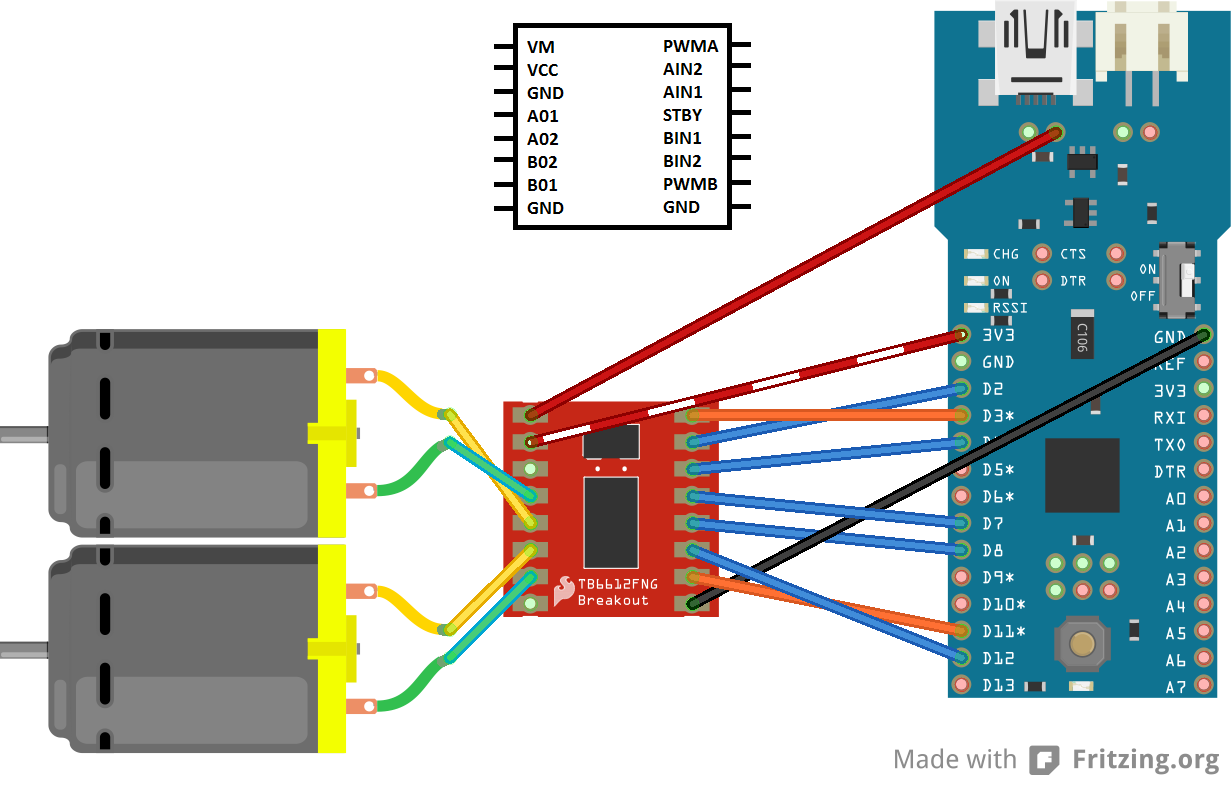
\includegraphics[width=0.8\textwidth]{./Figures/MODI/MODI_without_LED_bb.png}
		\rule{35em}{0.5pt}
	\caption[Conexión eléctrica Motor Driver 1A Dual TB6612FNG]{Diagrama de conexiones eléctricas para conectar Motor Driver 1A Dual TB6612FNG con motores DC y Arduino FIO.}
	\label{fig:TB6612FNG}
\end{figure}

%\FloatBarrier

%-----------------------------------
%	SUBSECTION 3
%-----------------------------------
\subsection{Batería LiPo y LED RGB}

Al comienzo se utilizaron baterías AAA para el robot, pero estas tienen el problema de que es necesario que el usuario las retire del robot para recargarlas. Por su parte las baterías LiPo permiten cargarse con el circuito de la Lipo Rider Pro y posee una alta densidad de carga, 2000mAh a 3.7V, que significa 10 horas de autonomía en funcionamiento continuo de los motores. Esta batería ayuda a cumplir con el \textbf{Requerimiento 5.}. Las pruebas de batería se realizaron solo utilizando los motores, la comunicación inalámbrica se desactivó para lograr 10.5 horas de funcionamiento continuo.

El \textbf{Requerimiento 7} se cumple incluyendo un LED RGB, que se puede controlar de manera simple para indicar los distintos estados en que puede encontrarse el robot. En la Figura \ref{fig:LED} se puede ver un diagrama de conexiones.

\begin{figure}[htbp]
	\centering
		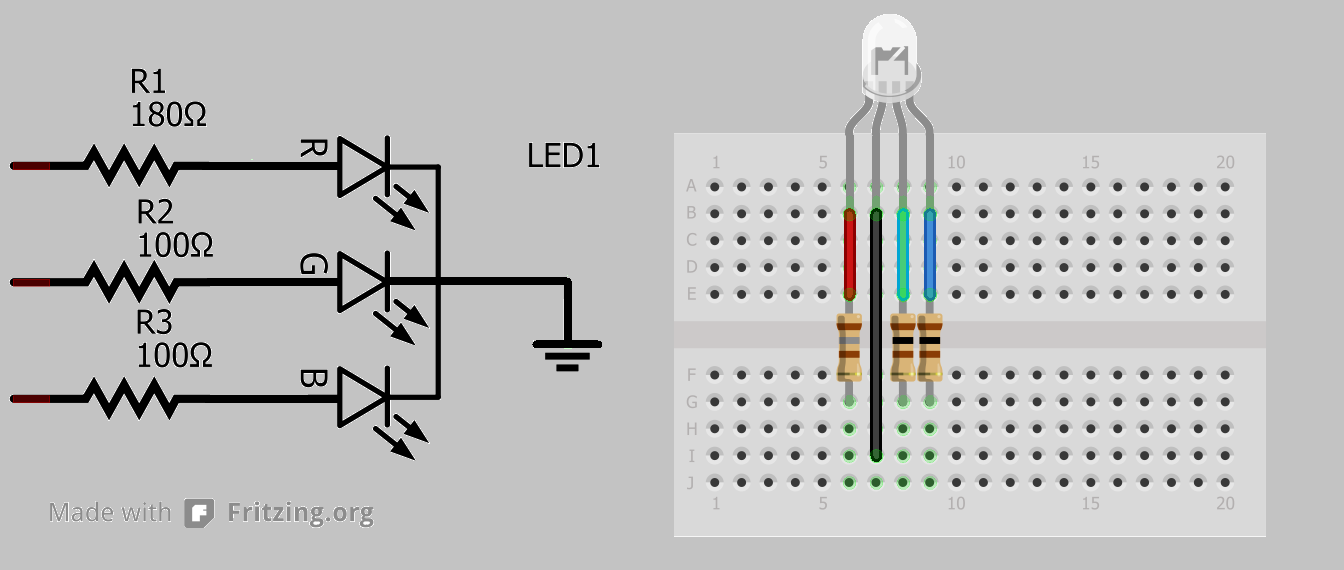
\includegraphics[width=0.8\textwidth]{./Figures/MODI/RGBLED.png}
		\rule{35em}{0.5pt}
	\caption[Conexión eléctrica LED RGB]{Diagrama de conexiones eléctricas para LED RGB. Para obtener un brillo óptimo se recomienda usar los valores de resistencias: 180 Ohm Rojo, 100 Ohm Verde, 100 Ohm Azul.}
	\label{fig:LED}
\end{figure}

\begin{figure}[htbp]
	\centering
		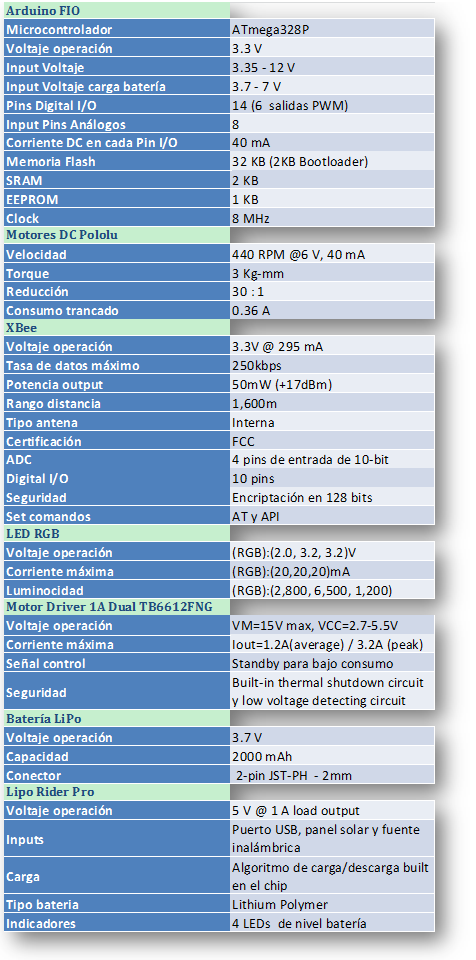
\includegraphics[width=0.8\textwidth]{./Figures/MODI/comparacionElo.png}
		\rule{35em}{0.5pt}
	\caption[Tabla caracteristicas más importantes de los componentes Eléctronicos]{Resumen de las características más importantes de los componentes electrónicos que tiene MODI.}
	\label{fig:TablaElo}
\end{figure}


%-----------------------------------
%	SECTION 4
%-----------------------------------

\section{Locomoción}
Existen distintas áreas donde se utilizan robots, dependiendo de la tarea a realizar es la movilidad que éste debe tener. Algunos tienen complejos sistemas como la plataforma del proyecto Atlas (The Agile Anthropomorphic Robot) de Boston Dynamics, Figura \ref{fig:Atlas}. En nuestro caso, sólo es necesario desplazarse sobre una superficie plana y por esto, en vez de tener costosos actuadores neumáticos, la solución más simple es contar con dos motores para poder tener un movimiento diferencial. Si se desea tener más información sobre los tipos de locomoción en robots con ruedas, ver esta pagina web\footnote{en.wikibooks.org/wiki/Robotics/Types\_of\_Robots/Wheeled}.


\begin{figure}[htbp]
	\centering
		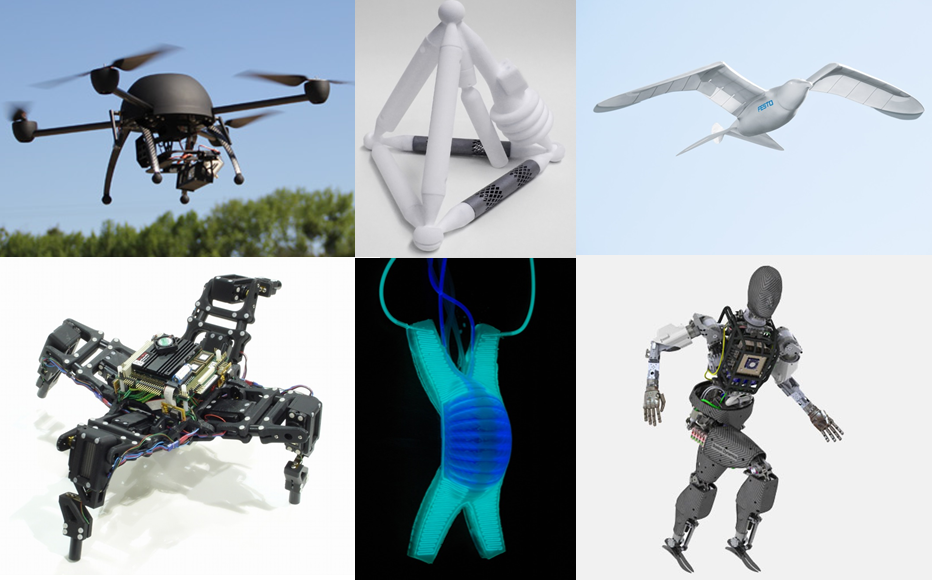
\includegraphics[width=\textwidth]{./Figures/robots.png}
		\rule{35em}{0.5pt}
	\caption[Robots]{Varios robots con distintos tipos de locomoción.}
	\label{fig:Atlas}
\end{figure}


Para moverse MODI tiene dos motores DC, ver Figura \ref{fig:compELO} f. Estos tienen una caja de reducción 30:1 que permiten aumentar el torque hasta 3 Kg-mm y disminuir la velocidad máxima hasta las 440 RPM. La Figura \ref{fig:DCMotor} a, muestra como se relaciona la velocidad y el consumo de corriente con el torque del motor.

\begin{figure}[htbp]
	\centering
		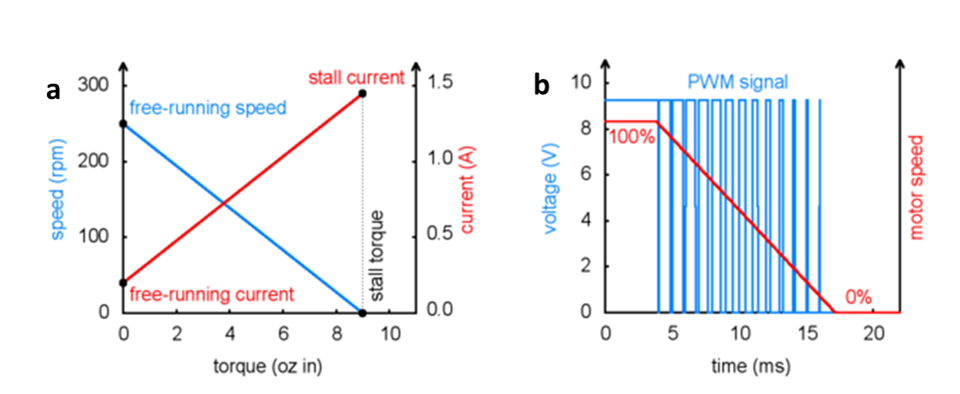
\includegraphics[width=0.8\textwidth]{./Figures/graficosMotores.png}
		\rule{35em}{0.5pt}
	\caption[Gráficos Motor DC]{a. Operación motores: Corriente, velocidad y torque. Imagen extraída de pololu.com, b. Control de velocidad PWM, se observa como disminuye la velocidad según ciclo de trabajo.}
	\label{fig:DCMotor}
\end{figure}

El control de velocidad de los motores se hace por medio de una señal PWM que se genera en el arduino. La señal PWM es periódica y se modifica solo su ciclo de trabajo, ver Figura \ref{fig:pwm}, que está relacionado con el valor medio de la señal. De manera que con una señal PWM con un ciclo de trabajo menor se obtiene un voltaje de salida menor, por ende una menor velocidad en el motor.  La Figura \ref{fig:DCMotor} b, relaciona el valor de la señal PWM como un voltaje con la velocidad del motor. Esta es una forma práctica de obtener salidas análogas desde una salida digital en Arduino. 
La potencia de los motores es controlada con el chip TB6612FNG, ver Figura \ref{fig:TB6612FNG}. En este diagrama se pueden ver dos cables naranjos, que son los que controlan la velocidad. En el Arduino se generan señales PWM en sus pins D3 y D11. Los valores que genera el Arduino para control de velocidad de los motores como representación interna de la señal PWM van desde 0 a 255, y además se puede controlar el sentido de giro según las salidas AIN y BIN. Por ejemplo para hacer que la rueda izquierda gire en sentido horario se debe dejar el pin AIN1 en 0 y AIN2 en 1 y la velocidad de ésta va a ser según el valor de la señal en PWMA, ver Figura \ref{fig:pwm} b. Para los distintos casos se puede ver la Figura \ref{fig:pwm} a, que indica los 3 movimientos que son: avanzar, avanzar hacia a la izquierda y girar en el eje. Aquí los números representan el período del ciclo de trabajo de la señal enviada por el Arduino al controlador de los motores. 

Se puede realizar un control más fino de la posición usando la información de posición del robot con un Control Proporcional, Integral y Diferencial (PID). El PID es para controlar un sistema realimentado, donde se calcula la desviación (error) entre un valor medido (la posición obtenida con el sistema de tracking) y el valor que se quiere obtener, para aplicar una acción correctora que ajuste el proceso. En este algoritmo hay tres parámetros distintos: el proporcional, el integral y el derivativo. El valor del parámetro proporcional produce una señal proporcional a la desviación de la salida del proceso. El integral elimina el problema del error en estado estacionario frente a perturbaciones de carga constante y el derivativo determina la reacción según el tiempo donde el error se produce. Estos tres parámetros permiten controlar la posición y/o orientación del robot MODI. Se recomienda ver este vídeo tutorial \footnote{http://www.youtube.com/watch?v=aE7RQNhwnPQ}. 

\begin{figure}[htbp]
	\centering
		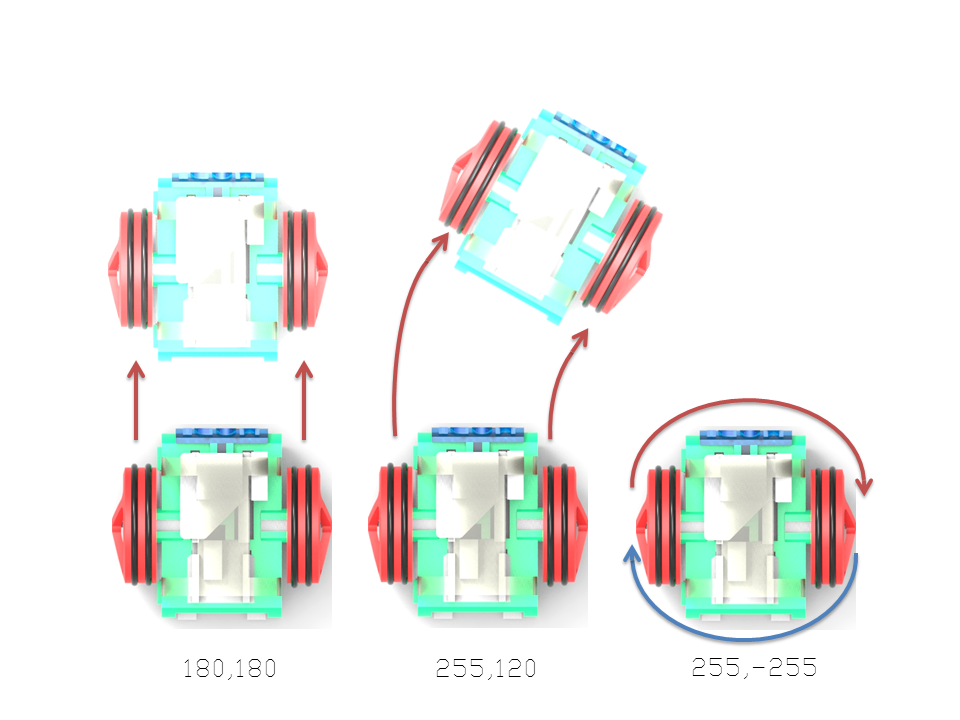
\includegraphics[width=\textwidth]{./Figures/MODI/pwm.png}
		\rule{35em}{0.5pt}
	\caption[Señal PWM]{Movimiento diferencial. A diferencia de un auto, MODI tiene dos motores que giran de forma independiente. Las distintas velocidades y sentido de giro determinan el ángulo para girar. Si se necesita solamente rotar los motores deben girar en sentidos opuestos. Se utiliza -255 en la última Figura para referirse a una señal PWM de 255 pero con sentido contrario.}
	\label{fig:pwm}
\end{figure}

%-----------------------------------
%	SECTION 5
%-----------------------------------
\section{Implementación}
La construcción de MODI fue motivada por una aplicación concreta, que es tener un grupo de robots controlables de forma independiente para hacer estudios del comportamiento del grupo. Para esto fue necesario montar un sistema simple con una cámara cenital que vigila  la posición y orientación de cada uno de ellos, como se puede ver en la Figura \ref{fig:setup}

El robot que se construyó para hacer las pruebas cuenta con un sistema externo de visión artificial que permite obtener posición y orientación de cada robot . Esto es necesario ya que como se mencionó, no existe ningún sensor interno del robot que le pueda ayudar a ubicarse en el espacio. Esta información es transmitida a cada robot por medio del protocolo \textit{zigbee} implementado en los chip XBee de la empresa Digi, ver Figura \ref{fig:compELO} b. Esto permite comunicar un alto número de robots, con muy poco consumo energético y de manera relativamente simple. Se escogió usar visión artificial sobre el sistema para bajar los costos individuales de los robots y XBee por ser el estándar en la industria en redes de sensores inalámbricos. Cabe destacar que los robots que existen en el mercado no incluyen XBee, y los que lo traen lo hacen como accesorio. 


%-----------------------------------
%	SECTION 6
%-----------------------------------

\subsection{Setup}

Para investigar el comportamiento colectivo de un grupo de robots, en el mundo real sin hacer uso de simuladores, es necesario contar con un lugar físico donde poder activar los robots. Además para simplificar cada uno de los robots, estos no tienen sensores internos por lo que hay una cámara montada sobre el plano de movimiento de estos, para hacer Seguimiento Visual. Esta información de coordenadas llega a un computador servidor que le indica a cada robot cómo moverse.
\begin{figure}[htbp]
	\centering
		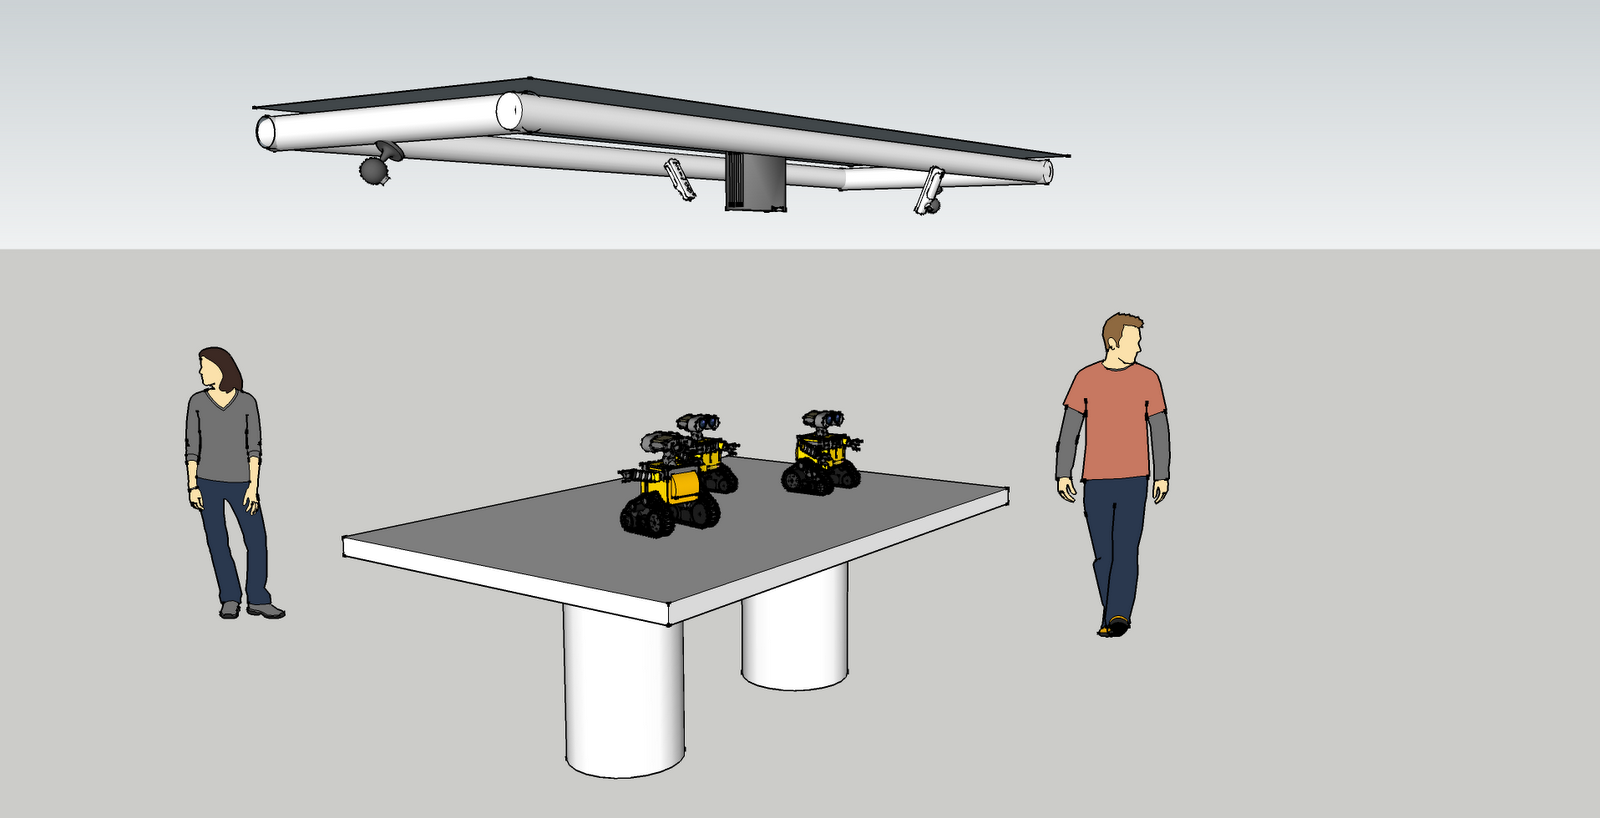
\includegraphics[width=\textwidth]{./Figures/setup.png}
		\rule{35em}{0.5pt}
	\caption[Setup Enjambre MODI]{Setup a montarse para hacer estudios de grupos de robots.}
	\label{fig:setup}
\end{figure}
%-----------------------------------
%	SUBSECTION 6
%-----------------------------------

\subsection{Software}

El software de MODI es bastante sencillo. Básicamente se configuraron todas las variables para cumplir con las conexiones eléctricas definidas en la Figura \ref{fig:Diagrama cables} y un puerto serial que está a la espera de comandos que indican acciones del robot. El puerto serie en MODI se configuró a una velocidad de 115200 y está esperando los caracteres ‘w’,’a’,’d’ y ‘s’, como Adelante, Izquierda, Derecha y Atrás respectivamente. 

Firmware y algunos ejemplos para testear funciones de manera individual se encuentran en el Git de MODI en Github. \footnote{https://github.com/FabLabUChile/modi}


\subsection{Tracking 2D}
Al igual que los seres vivos un robot necesita \textit{sentidos} o algún sistema sensorial para poder interactuar con su entorno. Estos pueden ser sensores IR para detectar objetos cercanos, cámaras o LASER para hacer un mapa del entorno o simplemente un pulsador que sea presionado cada vez que el robot colisiona. Para bajar costos, MODI actualmente no cuenta con sensores “onBoard”. Cada robot es comandado por un sistema que le dice donde está él, donde están los demás, y los límites del área de trabajo. Se diseñó de esta manera para simplificar la programación de cada robot. En la Figura \ref{fig:FidTracking} se diagrama el funcionamiento del sistema de traking 2D.


\begin{figure}[htbp]
	\centering
		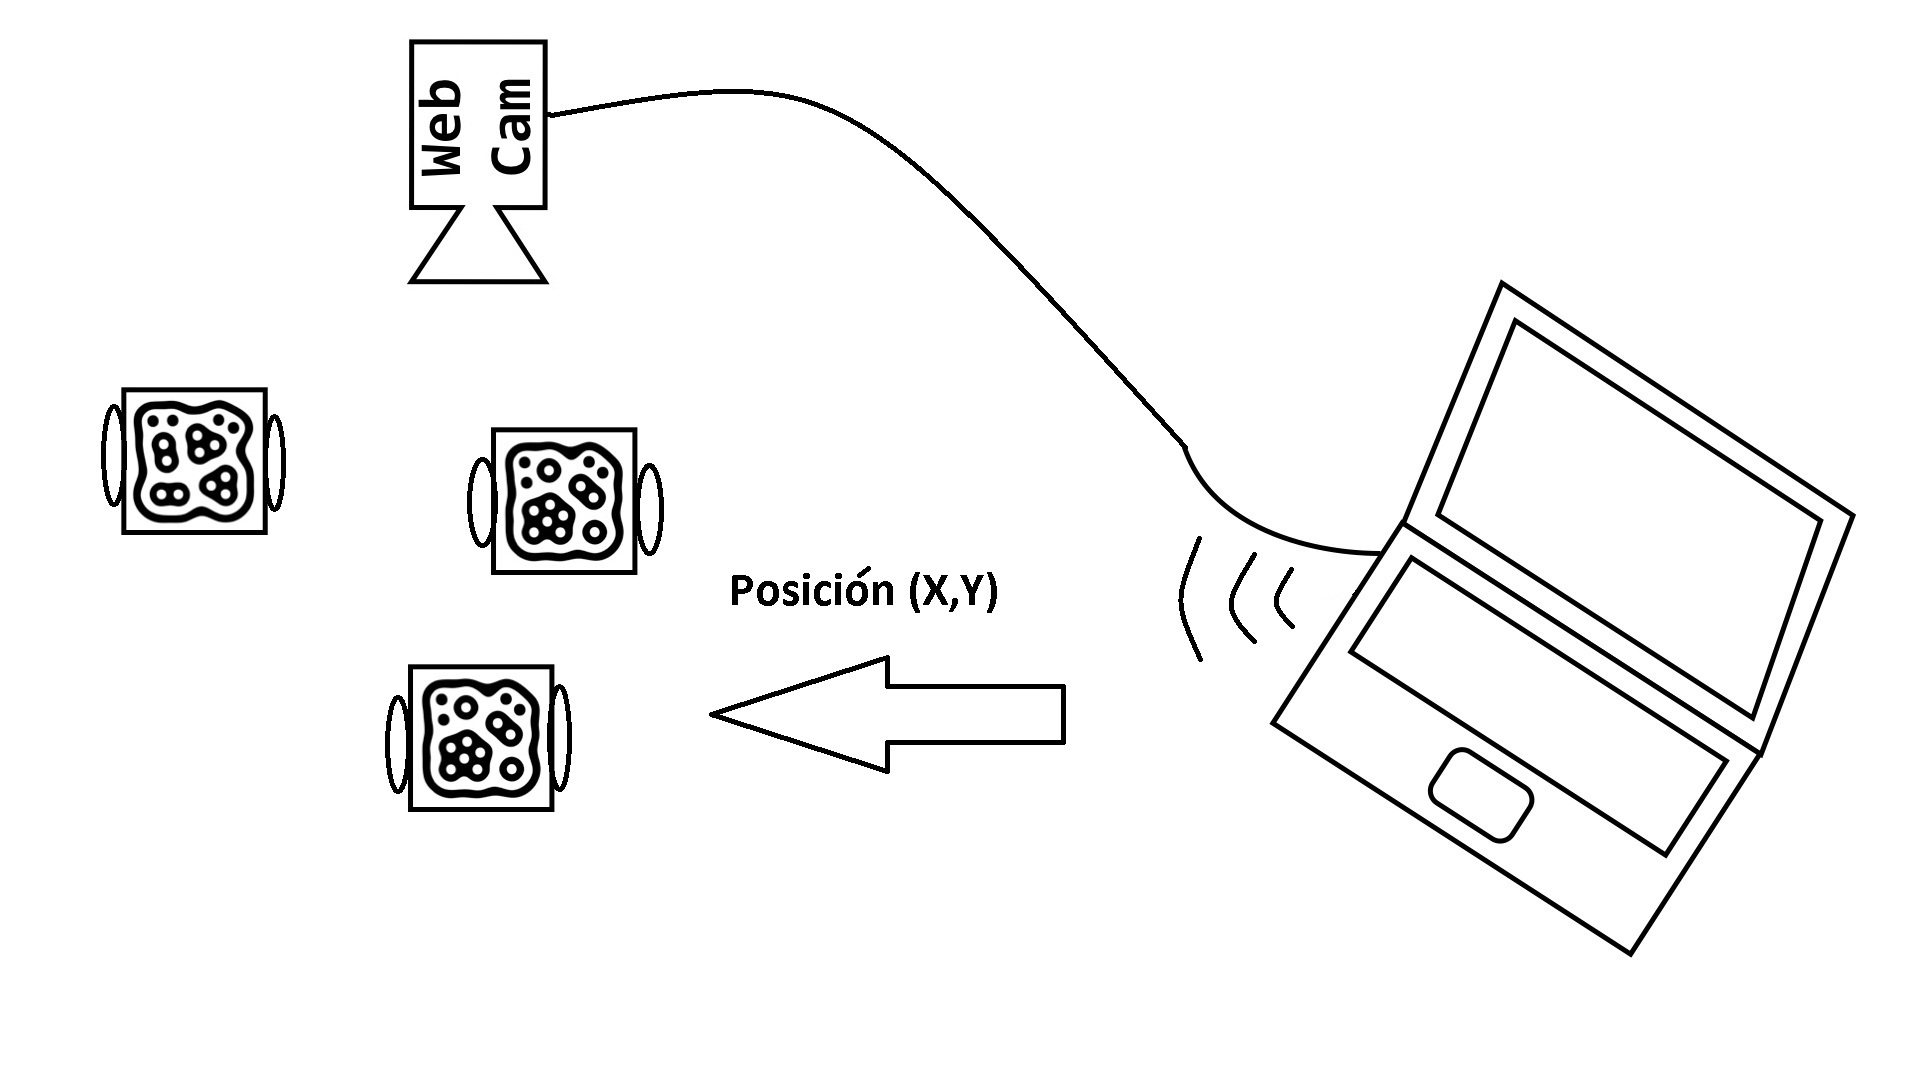
\includegraphics[width=0.65\textwidth]{./Figures/MODI/fidPosicion.jpg}
		\rule{35em}{0.5pt}
	\caption[Diagrama Fiduciales]{Diagrama que explica el funcionamiento de tracking por medio de tags fiduciales.}
	\label{fig:FidTracking}
\end{figure}

reacTIVision \cite{kaltenbrunner2007reactivision} es un framework Open Source, cross-platform, para realizar tracking rápido y robusto de tags fiduciales, pegadas a objetos físicos, ver Figura \ref{fig:Fiducial}. Ha sido diseñado como un toolkit para el desarrollo rápido de multi-touch interactive surfaces. Este framework fue desarrollado por Martin Kaltenbrunner y Ross Bencina en el Music Technology Group de la universidad de Pompeu Fabra en Barcelona, España. reacTIVision fue diseñado como sensor principal de la Reactable, un sintetizador modular tangible que ha marcado los standards en lo que a aplicaciones multitouch se refiere. 
Esta alternativa debe ir acompañada de otros elementos, como la cámara y el computador en el cual se ejecuta el software. Con estos elementos mediante un protocolo llamado TUIO, disponible como biblioteca en los lenguajes de programación más populares, se puede obtener: la posición, orientación e identificador de cada robot, cumpliendo con el \textbf{Requerimiento 6}. Con reacTIVision es posible detectar hasta 216 tag fiduciales a una velocidad de 50 fps a una resolución de 640 x 480.




\begin{figure}[htbp]
	\centering
		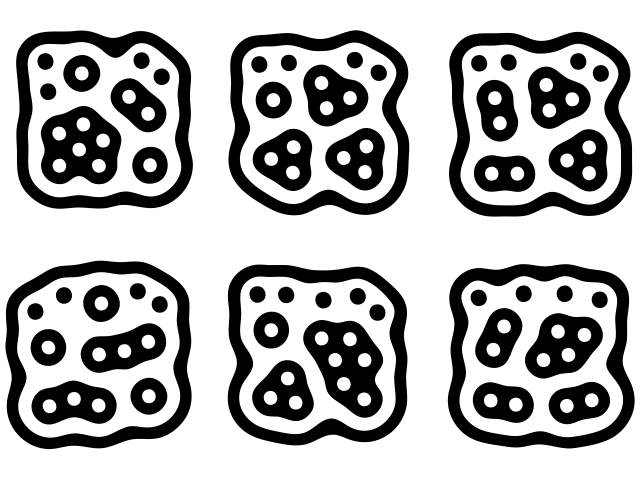
\includegraphics[width=0.65\textwidth]{./Figures/MODI/fiducial.png}
		\rule{35em}{0.5pt}
	\caption[Fiduciales usados como tag en reacTIVision]{Códigos fiduciales utilizados en reacTIVision. Estos códigos aunque parecen algo extraños para los seres humanos están diseñados de tal forma que es muy fácil diferenciar unos de otros y además obtener su orientación y posición en un software de análisis de imágenes. Se tiene un total de 216 configuraciones posibles de códigos.}
	\label{fig:Fiducial}
\end{figure}



%-----------------------------------
%	SECTION 7
%-----------------------------------

\subsection{Lista de Materiales (BOM)}

Con un precio total de 180 USD, Figura \ref{fig:BOM}, MODI se propone como una alternativa económica para construir un robot de desplazamiento diferencial. Pensando en comprar desde Chile, son tres las tiendas en que se cotizaron los componentes. Es posible comprar todo desde internet. Para más detalles sobre la Lista de materiales, o en ingles Bill Of Materials (BOM), ver link \footnote{http://kitbom.com/otrab/modi}.
\begin{figure}[htbp]
	\centering
		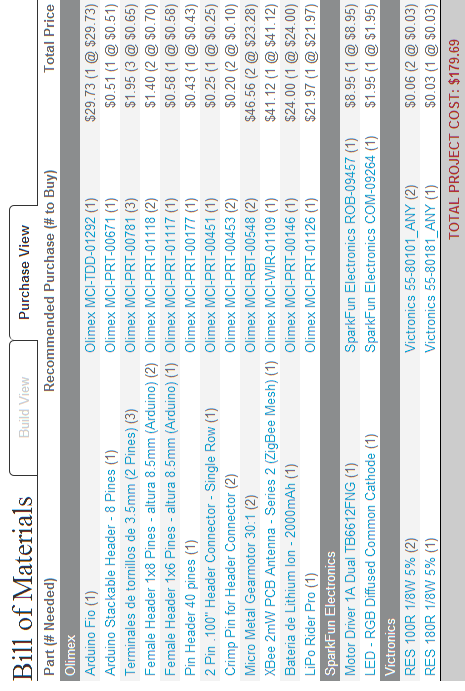
\includegraphics[width=\textwidth]{./Figures/MODI/kitbom.png}
		\rule{35em}{0.5pt}
	\caption[Bill Of Materials]{Lista de materiales a comprar para construir un robot MODI, la versión online de este BOM se puede ver en http://kitbom.com/otrab/modi}
	\label{fig:BOM}
\end{figure}

Luego de haber seleccionado los componentes se incluye la tabla en la Figura \ref{fig:Tabla robots MODI} que compara al robot MODI con los otros robots estudiados en el capítulo 3.

\begin{figure}[htbp]
	\centering
		\includegraphics[width=0.6\textwidth]{./Figures/tabla_robots_modi.png}
		\rule{35em}{0.5pt}
	\caption[Tabla comparativa robots MODI]{En esta tabla se comparan las características principales del robot MODI con los robots: kilobot, e-puck y 3pi.}
	\label{fig:Tabla robots MODI}
\end{figure} 
% Chapter Template

\chapter{Aplicaciones de MODI} % Main chapter title

\label{Chapter6} % Change X to a consecutive number; for referencing this chapter elsewhere, use \ref{ChapterX}

\lhead{Capitulo 6. \emph{Aplicaciones de MODI}} % Change X to a consecutive number; this is for the header on each page - perhaps a shortened title

%----------------------------------------------------------------------------------------
%	SECTION 1
%----------------------------------------------------------------------------------------

\section{Educación}

Un enjambre de robots puede presentar muchas ventajas dentro del aula. Si se tiene un sistema de fácil uso para los alumnos, el profesor puede asignar una tarea a un grupo de estudiantes donde cada uno tiene la responsabilidad de controlar o programar un robot para que el conjunto logre una meta determinada como ordenar unos bloques o hacerse cargo de regar un pequeño huerto. Abusando un poco del concepto de la colectividad, incluso pueden generarse tareas donde cada colegio se especializa en un tipo de tareas para luego juntar los distintos robots y probar cómo interactúan.

Tener un setup con robots que demuestren un comportamiento colectivo puede ser muy ventajoso para promover el aprendizaje de roles sociales si la docente a cargo programa los robot para que tengan distintos roles como Líder y participante. Este mismo juego de roles puede ayudar a los niños a generar estrategias y herramientas para enfrentarse al mundo. En síntesis haciendo juegos para los niños con los robots se puede tener su atención para reforzar su educación y favorecer en el desarrollo de habilidades y competencias. 

\section{Usos Militar}

Con un enjambre de robots, se puede simular una situación de catástrofe, donde es necesario poder desplegar un grupo de robots para hacer una tarea de reconocimiento y así poder buscar personas heridas o atrapadas.
Imaginemos una situación hipotética donde un edificio es destruido, la búsqueda de sobrevivientes no es una tarea fácil, implica que rescatistas ingresen al lugar corriendo grave peligro, usualmente buscando a las víctimas en condiciones de poca visibilidad. Esto mismo podría ser ejecutado por un enjambre robótico que esté programado para buscar gente y que de manera colectiva recorra un área mucho mayor que 2 o 3 personas. Incluso un robot del mismo enjambre puede fallar, pero al ser un sistema distribuido el enjambre continúa funcionando, es un sistema muy robusto.

\section{Usos Doméstico}

Existen las aspiradoras Roomba, que sin necesidad de un operario humano pueden aspirar nuestras casas. Ellas recorren nuestro hogar y gracias a sus sensores pueden auto generar un mapa del entorno. Este modelo del hogar puede hacerse mucho más rápido si en vez de tener un solo robot, se tienen 20. El mismo concepto se puede aplicar en seguridad del hogar, donde se pueden tener varios mini robots haciendo rondas en el perímetro de nuestra casa y en forma colectiva abarcan lo más posible. Todas estas situaciones se pueden simular con los robot MODI.

% Chapter Template

\chapter{Mejoras futuras y Conclusiones} % Main chapter title

\label{ChapterX} % Change X to a consecutive number; for referencing this chapter elsewhere, use \ref{ChapterX}

\lhead{Capitulo 4. \emph{Conclusiones}} % Change X to a consecutive number; this is for the header on each page - perhaps a shortened title

%----------------------------------------------------------------------------------------
%	SECTION 1
%----------------------------------------------------------------------------------------

\section{Mejoras futuras}

Son muchas las mejoras que pueden hacerse en MODI, el diseño es un cuento de nunca acabar. En esta primera versión se priorizaron los requerimientos para construir un enjambre, dejando un poco de lado algunos aspectos que pueden ser importantes pero que no son parte fundamental del proyecto.

A continuación se explican algunas de las mejoras que pueden realizarse y como implementarlas.


%-----------------------------------
%	SUBSECTION 1
%-----------------------------------
\subsection{Encoders}
Una de las características claves de MODI es que hace uso de un tag fiducial, para poder tener información de la posición y orientación de cada robot. Con esto es posible controlar la navegación del robot, pero debido al roce o deslizamiento de las ruedas, se pueden mover diferente a lo esperado, provocando un error en la posición final. Si se necesita tener un control más fino sobre cada uno de los motores es fundamental incluir encoders en las ruedas. Por los motores que se tiene, se sugiere usar los enconders Pololu \footnote{http://www.pololu.com/catalog/product/1217}. Esta mejora no se implementó ya que implica modificar el PCB MODI para poder conectar los encoders al micro controlador Arduino.

%-----------------------------------
%	SUBSECTION 2
%-----------------------------------
\subsection{Cables incrustados y Soporte motor}
Es ideal que el mismo chasis del robot pueda contener las conexiones eléctricas y así reducir aún más la dificultad de ensamblado. Es por esto que se propuso un diseño con pequeños canales para incrustar los cables de los motores y que, además permite usar pins en los extremos que sirven para conectar eléctricamente los motores. Se puede ver en la Figura \ref{fig:Cables incrustados} esta idea, junto con una versión mejorada del soporte para los motores Pololu, que son motores ampliamente usados en robotica.
Pese a ser una mejora simple de incluir en el diseño del chasis de MODI, se decidio dejar este punto como mejora a futuro ya que es necesario hacer una investigación sobre el tipo de conectores electricos a usar y si utilizar cables u otro tipo de material conductivo en los canales.

\begin{figure}[htbp]
	\centering
		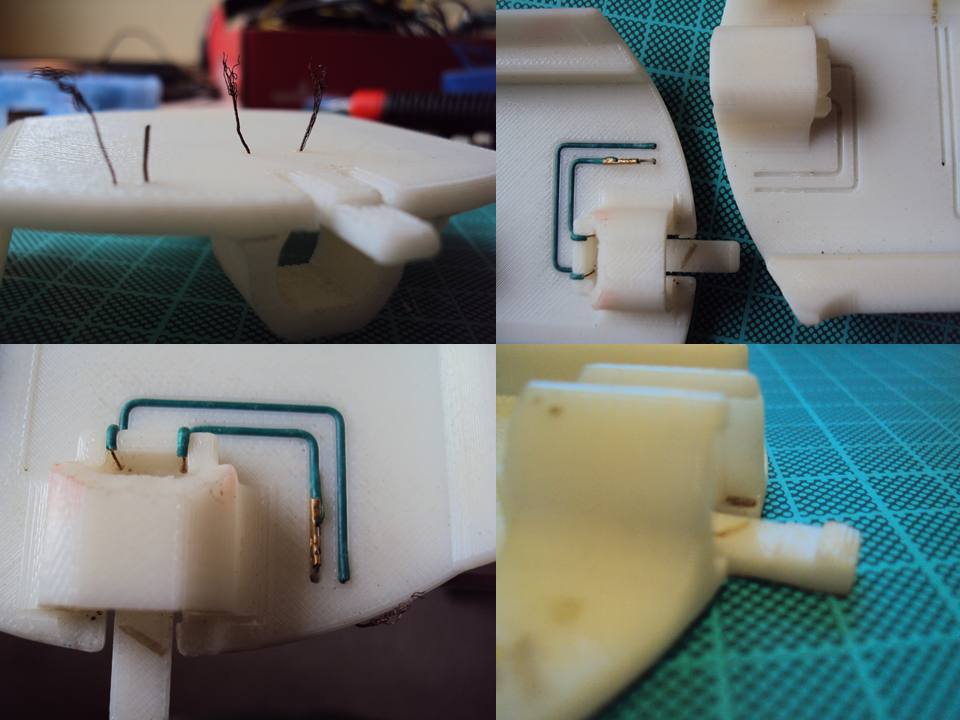
\includegraphics[width=\textwidth]{./Pictures/wires.png}
		\rule{35em}{0.5pt}
	\caption[Cables incrustados y Soporte motor]{Diseño propuesto por Dr. Pablo Prieto para optimizar el cableado eléctrico en el chasis de MODI. También se puede ver otra versión del Soporte motor, que incluye una pestaña que afirma al motor.}
	\label{fig:Cables incrustados}
\end{figure}	






%-----------------------------------
%	SUBSECTION 4
%-----------------------------------

\subsection{Una PCB para todo}

Para simplificar las conexiones del robot es necesario diseñar un nuevo PCB que incluya: Arduino, Driver motores y socket XBee, componentes electrónicos de MODI en Figura \ref{fig:compELO}. Esto debido a que demanda cierto tiempo tener que hacer los conectores necesarios para que se comuniquen entre sí. Tener este PCB implica bajar los costos de fabricación ya que es una sola PCB que se manda a fabricar, en vez de comprar tres en el mercado. Cabe destacar que esto debe ser un trabajo relativamente simple ya que todas las placas utilizadas son Open Source, lo que implica que sus archivos de diseño se encuentran completamente libre para su distribución, estudio, modificación y uso.


%-----------------------------------
%	SUBSECTION 2
%-----------------------------------

\subsection{Módulo de carga inalámbrica}
La elección de tener un Lipo Rider Pro en el robot en parte considera el uso de diversas formas de carga de energía. De forma simple se puede conectar un panel solar con conector JST 2.0, y en este mismo conector se puede poner un módulo de carga inalámbrica como el que vende SeeedStudio \footnote{http://www.seeedstudio.com/depot/wireless-charging-module-p-1354.html}. Estas alternativas permiten tener un setup de robots funcionando ininterrumpidamente ya que no es necesario intervenir los robots para cargar sus baterías. 


%----------------------------------------------------------------------------------------
%	SECTION 2
%----------------------------------------------------------------------------------------

\section{Conclusiones}
Diseñar un robot es una hermosa misión que implica desarrollar e integrar habilidades en varias áreas. Por lo mismo es necesario tener un equipo multidisciplinario que pueda abordar el problema desde distintas perspectivas. Para este trabajo fue fundamental contar con visiones expertas en robótica, diseño y biología-electrónica para hacer que MODI sea un gran proyecto que en un futuro pueda involucrar a mucha gente.

Con el equipo de trabajo armado los desafíos son adaptarse a la realidad nacional, donde se tienen menos recursos, tanto monetarios como de \textit{materias primas electrónicas}. Por esto es necesario lograr  hacer pruebas a pequeña escala para tomar decisiones en el diseño. Una herramienta fundamental para hacer pruebas a pequeña escala son las impresoras 3D que permiten en un día probar varios modelos distintos y hacer pruebas que no implican grandes pérdidas. Además de las impresoras 3D, con acceso a una Router CNC y un laboratorio básico de electrónica se puede hacer un producto que puede competir en el mercado.

Otras herramientas importantes en este trabajo son las tecnologías Open Source, que más bien es una filosofía donde se entrega de manera libre a la comunidad trabajo de gran calidad para que sea \textit{utilizado, modificado y compartido}. Muchos de los elementos importantes de MODI son Open Source, lo que implica que MODI también es un proyecto Open. Gracias a que se incluyeron estas tecnologías se pudo reducir el tiempo de desarrollo drásticamente.

MODI como robot es simple, tan simple que si no se tienen aplicaciones concretas el proyecto puede diluirse. Es importante hacer difusión del proyecto y en especial trabajar con áreas que estén algo más alejadas de la electrónica, que son las más beneficiadas con MODI ya que al tener una curva de aprendizaje rápida, permite enfocarse sólo en la tarea fundamental y dejar de lado los aspectos técnicos que implican construir un robot. Se recomienda que gente del área de la zoología, biología, visión, psicología, educación, informática, por nombrar algunas, se les capacite y facilite el acceso a esta plataforma que puede ayudar a desentrañar aspectos claves de nuestra naturaleza. En comparación con los otros robots estudiados, MODI es capaz de cumplir con los requerimientos del proyecto a una fracción del costo y cualquiera con acceso a un FabLab puede construir uno.

Un ejemplo de aplicación en otras áreas es el uso de este robot en educación. Muchos de los elementos incluidos en MODI, ya sea software o hardware, son grandes herramientas que pueden ser útiles para resolver otros desafíos tecnológicos como hacer uso de sensores inalámbricos o trabajar con energía solar, que gracias a la simplicidad del proyecto quedan expuesto de manera clara y modular. Es por esto que MODI es ideal como robot para introducirse en la robótica, permitiendo al usuario de manera libre estudiar todas sus características en la medida que lo necesite. De lograrse esto, se tendría un gran impacto educacional en Chile ya que MODI podrá ser la puerta de entrada para introducir fácilmente la robótica en el sistema educacional chileno.


%----------------------------------------------------------------------------------------
%	THESIS CONTENT - APPENDICES
%----------------------------------------------------------------------------------------

\addtocontents{toc}{\vspace{2em}} % Add a gap in the Contents, for aesthetics

\appendix % Cue to tell LaTeX that the following 'chapters' are Appendices

% Include the appendices of the thesis as separate files from the Appendices folder
% Uncomment the lines as you write the Appendices

% Appendix A

\chapter{} % Main appendix title

\label{AppendixA} % For referencing this appendix elsewhere, use \ref{AppendixA}

\lhead{Apéndice} % This is for the header on each page - perhaps a shortened title

Algunas cosas interesantes que faltó incluir en el trabajo:
Primero una imagen de algunas versiones de MODI, que fueron posibles por tener acceso a impresoras 3D ya que hacen muy simple el proceso de hacer cambios en los prototipos.

\begin{figure}[htbp]
	\centering
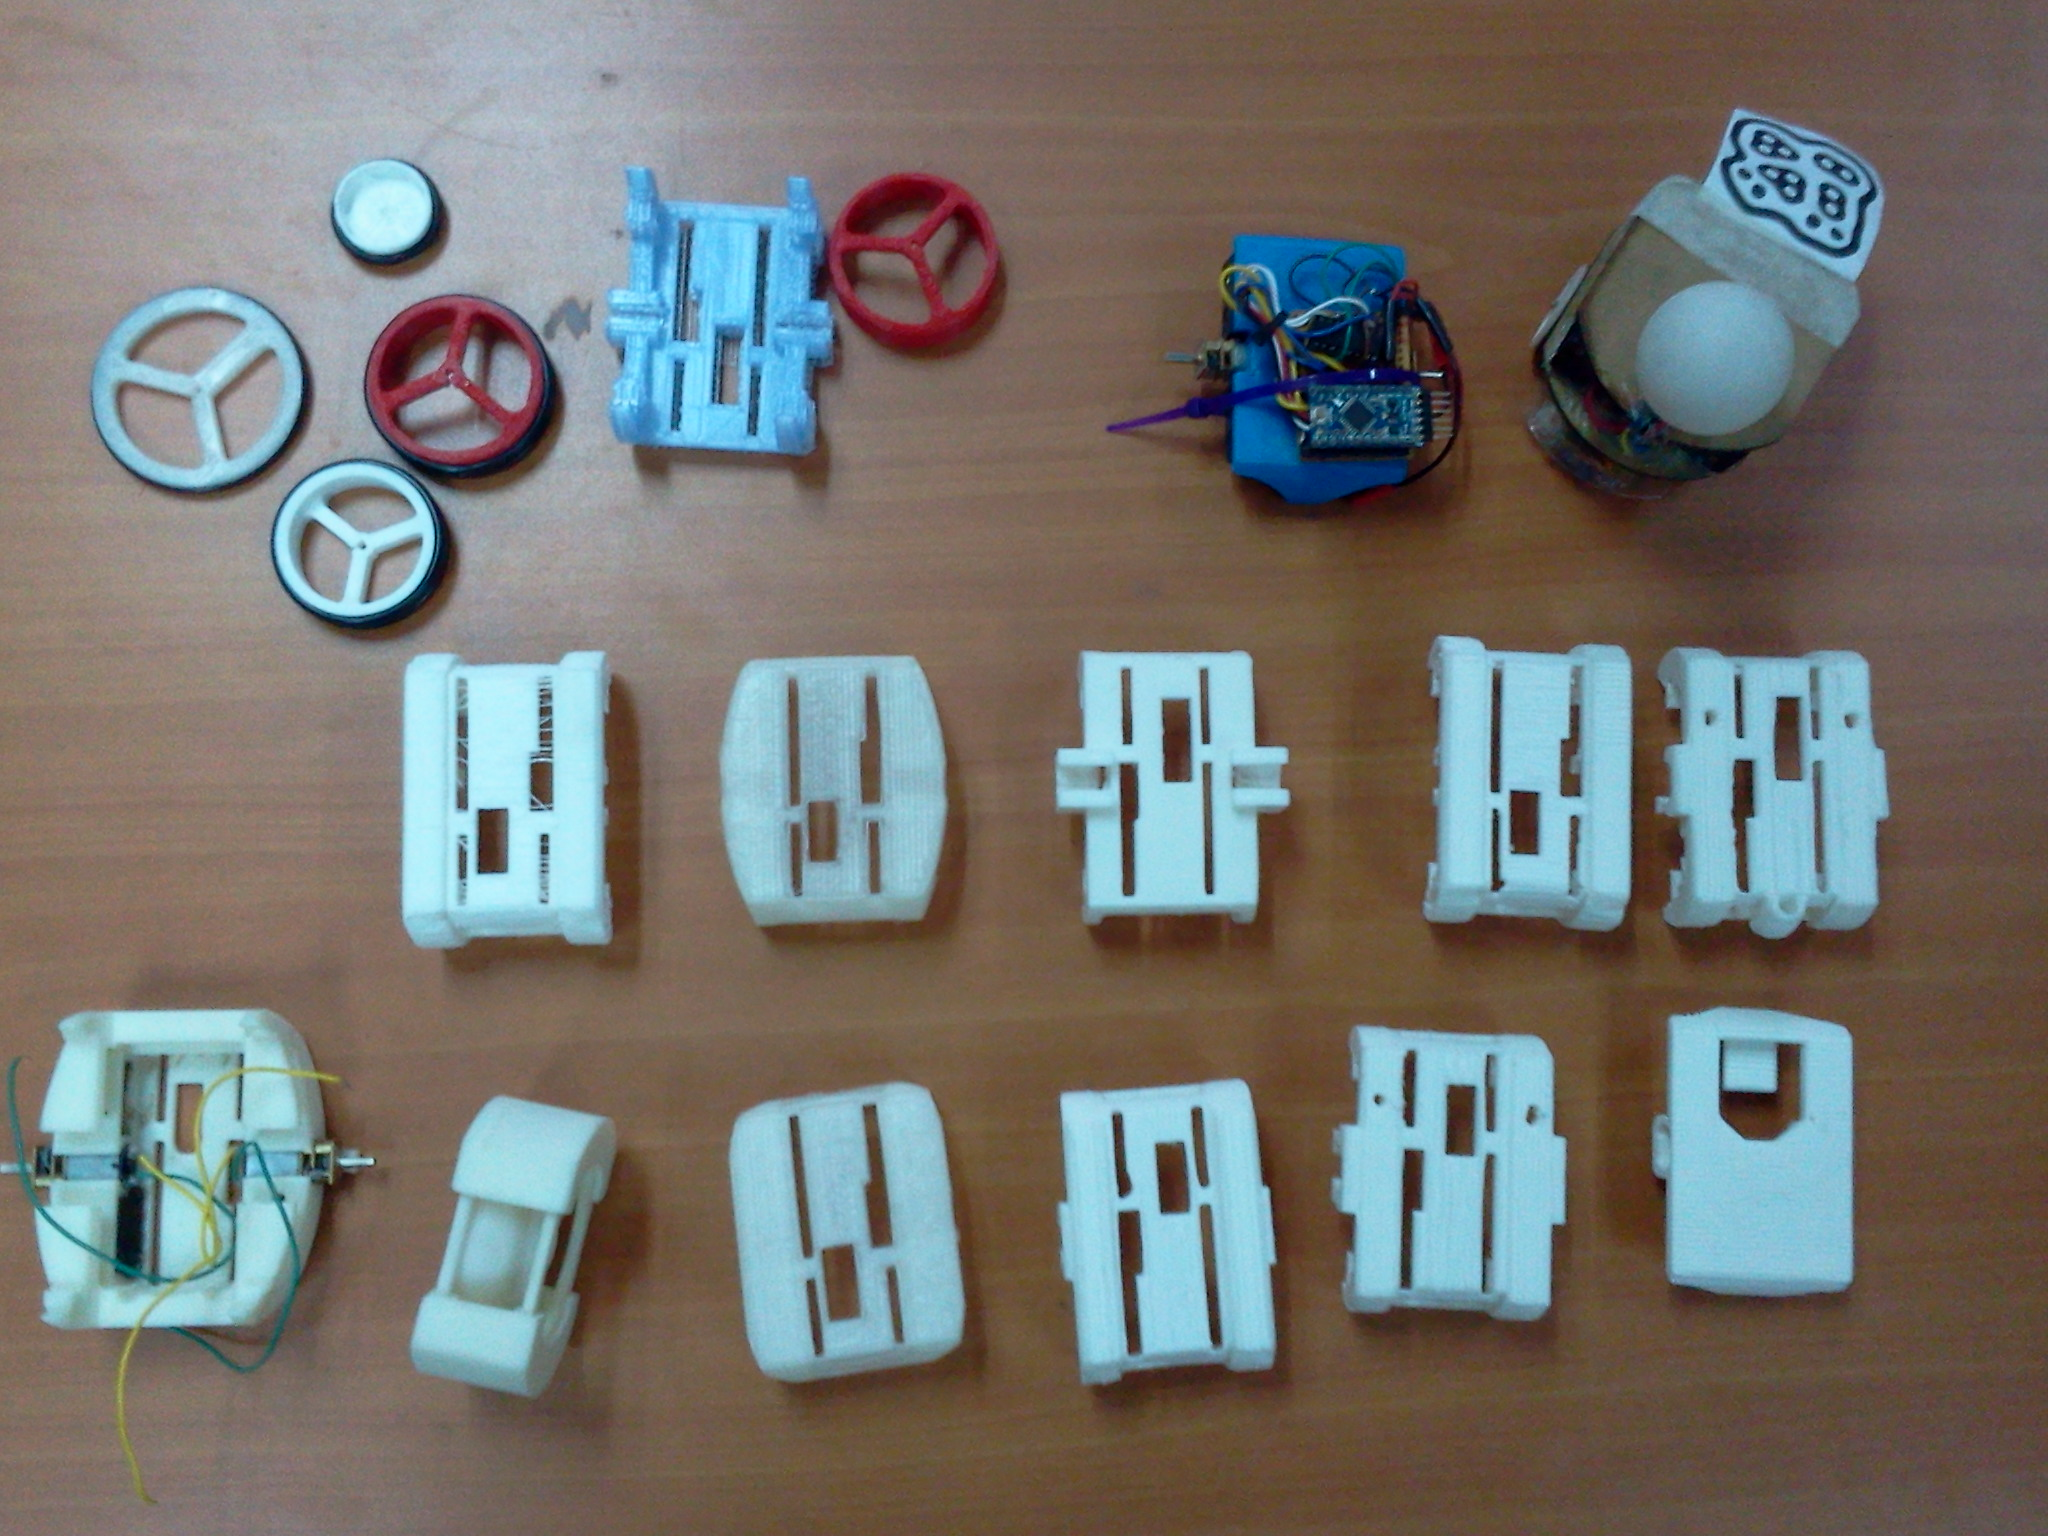
\includegraphics[width=\textwidth]{./Pictures/historia.jpg}
		\rule{35em}{0.5pt}
	\caption[Historia de construcción]{Algunos de los modelos que se construyeron para llegar a la versión final de MODI.}
	\label{fig:Historia}
\end{figure}

\newpage 
Lo segundo es el PCB diseñado para MODI que une el controlador de motores al arduino FIO y permite contectar un LED RGB.
\begin{figure}[htbp]
	\centering
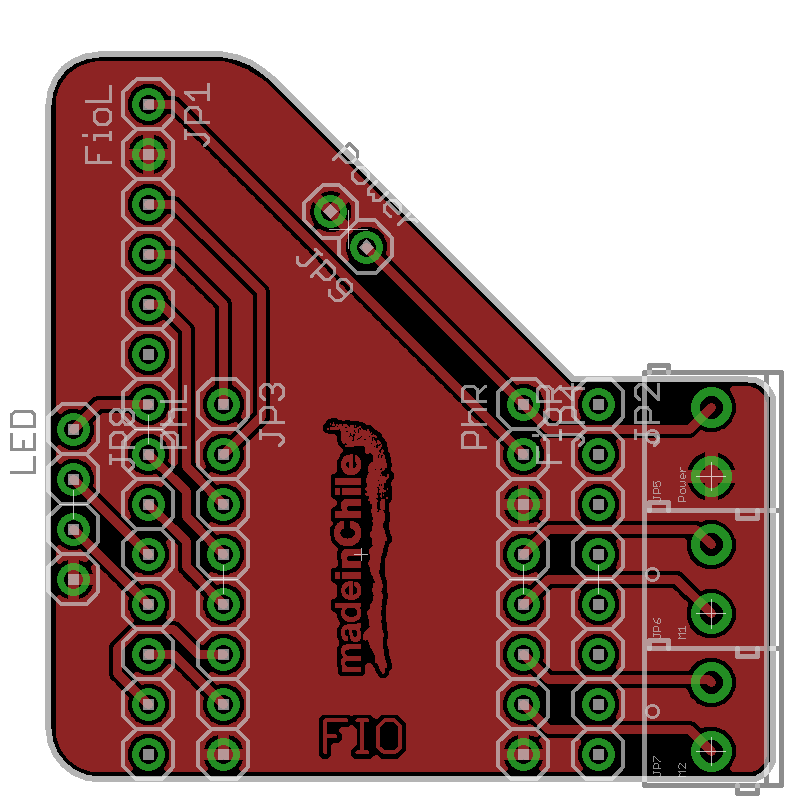
\includegraphics[width=\textwidth]{./Figures/MODI/pcbmodi.png}
		\rule{35em}{0.5pt}
	\caption[PCB MODI]{PCB diseñada para conectar motores, LED RGB al Arduino FIO.}
	\label{fig:PCBA}
\end{figure}

%\input{./Appendices/AppendixB}
%\input{./Appendices/AppendixC}

\addtocontents{toc}{\vspace{2em}} % Add a gap in the Contents, for aesthetics

\backmatter

%----------------------------------------------------------------------------------------
%	BIBLIOGRAPHY
%----------------------------------------------------------------------------------------

\label{Bibliography}
%Renombrar pagina
\renewcommand{\bibname}{Referencias}
\renewcommand{\refname}{Referencias}

\lhead{\emph{Bibliography}} % Change the page header to say "Bibliography"

\bibliographystyle{unsrtnat} % Use the "unsrtnat" BibTeX style for formatting the Bibliography

\bibliography{Bibliography} % The references (bibliography) information are stored in the file named "Bibliography.bib"

\end{document}
